\chapter{Pictorial Representation}\label{ch:pictorial}

% Box-drawing glyphs for verbatim character-grid drawings (pdfLaTeX has no such glyphs).
\newcommand{\pgc}[1]{\makebox[0.525em][l]{\begin{tikzpicture}[overlay,x=0.525em,y=\baselineskip,line width=0.4pt]#1\end{tikzpicture}}}
\newcommand{\pgL}{\draw (-0.05,0.22)--(0.5,0.22);}
\newcommand{\pgR}{\draw (0.5,0.22)--(1.05,0.22);}
\newcommand{\pgU}[1]{\draw[line width=#1] (0.5,0.22)--(0.5,0.75);}
\newcommand{\pgD}[1]{\draw[line width=#1] (0.5,0.22)--(0.5,-0.31);}
\newcommand{\gH}{\pgc{\pgL\pgR}}
\newcommand{\gV}{\pgc{\pgU{0.4pt}\pgD{0.4pt}}}
\newcommand{\gRD}{\pgc{\pgR\pgD{0.4pt}}}
\newcommand{\gLD}{\pgc{\pgL\pgD{0.4pt}}}
\newcommand{\gRU}{\pgc{\pgR\pgU{0.4pt}}}
\newcommand{\gLU}{\pgc{\pgL\pgU{0.4pt}}}
\newcommand{\gX}{\pgc{\pgL\pgR\pgU{0.4pt}\pgD{0.4pt}}}
\newcommand{\gHV}{\pgc{\pgU{1.2pt}\pgD{1.2pt}}}
\newcommand{\gHRD}{\pgc{\pgR\pgD{1.2pt}}}
\newcommand{\gHRU}{\pgc{\pgR\pgU{1.2pt}}}
\newcommand{\gHRV}{\pgc{\pgR\pgU{1.2pt}\pgD{1.2pt}}}
\newcommand{\gHLD}{\pgc{\pgL\pgD{1.2pt}}}
\newcommand{\gHLU}{\pgc{\pgL\pgU{1.2pt}}}
\newcommand{\gHLV}{\pgc{\pgL\pgU{1.2pt}\pgD{1.2pt}}}
\newcommand{\gDH}{\pgc{\draw (-0.05,0.31)--(1.05,0.31); \draw (-0.05,0.13)--(1.05,0.13);}}
\newcommand{\gDV}{\pgc{\draw (0.3,-0.31)--(0.3,0.75); \draw (0.7,-0.31)--(0.7,0.75);}}
\newcommand{\gDHx}{\pgc{\draw (-0.05,0.31)--(1.05,0.31); \draw (-0.05,0.13)--(1.05,0.13); \draw (0.5,-0.31)--(0.5,0.75);}}
\newcommand{\gDVx}{\pgc{\draw (0.3,-0.31)--(0.3,0.75); \draw (0.7,-0.31)--(0.7,0.75); \draw (-0.05,0.22)--(1.05,0.22);}}
\newcommand{\gDTL}{\pgc{\draw (1.05,0.31)--(0.3,0.31)--(0.3,-0.31); \draw (1.05,0.13)--(0.7,0.13)--(0.7,-0.31);}}
\newcommand{\gDTR}{\pgc{\draw (-0.05,0.31)--(0.7,0.31)--(0.7,-0.31); \draw (-0.05,0.13)--(0.3,0.13)--(0.3,-0.31);}}
\newcommand{\gDBL}{\pgc{\draw (1.05,0.13)--(0.3,0.13)--(0.3,0.75); \draw (1.05,0.31)--(0.7,0.31)--(0.7,0.75);}}
\newcommand{\gDBR}{\pgc{\draw (-0.05,0.13)--(0.7,0.13)--(0.7,0.75); \draw (-0.05,0.31)--(0.3,0.31)--(0.3,0.75);}}
\newcommand{\gcirc}[1]{\pgc{\draw (0.5,0.24) circle[radius=0.27em]; \node[font=\fontsize{4}{4}\selectfont\sffamily,inner sep=0pt] at (0.5,0.24) {#1};}}
\newcommand{\gZ}{\gcirc{Z}}
\newcommand{\gXs}{\gcirc{X}}
\newcommand{\gG}{\pgc{\draw (0,0.22)--(0.3,0.22); \draw[line width=0.6pt] (0.3,0.0)--(0.3,0.44); \draw[line width=0.6pt] (0.55,0.07)--(0.55,0.37); \draw[line width=0.6pt] (0.8,0.14)--(0.8,0.30);}}
\newcommand{\gtri}[1]{\makebox[0.525em]{\scalebox{0.62}{$#1$}}}
\lstdefinestyle{pgrid}{language={},basicstyle=\ttfamily\small,columns=fixed,basewidth=0.525em,
  keepspaces=true,breaklines=false,frame=single,
  literate={─}{{\gH}}1 {│}{{\gV}}1 {┌}{{\gRD}}1 {┐}{{\gLD}}1 {└}{{\gRU}}1 {┘}{{\gLU}}1
    {┼}{{\gX}}1 {┃}{{\gHV}}1 {┎}{{\gHRD}}1 {┖}{{\gHRU}}1 {┠}{{\gHRV}}1 {┒}{{\gHLD}}1
    {┚}{{\gHLU}}1 {┨}{{\gHLV}}1 {═}{{\gDH}}1 {║}{{\gDV}}1 {╪}{{\gDHx}}1 {╫}{{\gDVx}}1
    {╔}{{\gDTL}}1 {╗}{{\gDTR}}1 {╚}{{\gDBL}}1 {╝}{{\gDBR}}1 {Ⓩ}{{\gZ}}1 {Ⓧ}{{\gXs}}1
    {⏚}{{\gG}}1 {◀}{{\gtri{\blacktriangleleft}}}1 {▶}{{\gtri{\blacktriangleright}}}1
    {▷}{{\gtri{\triangleright}}}1 {⊳}{{\gtri{\vartriangleright}}}1 {⊲}{{\gtri{\vartriangleleft}}}1
    {⁻}{{$^{-}$}}1 {¹}{{$^{1}$}}1 {√}{{$\surd$}}1 {·}{{$\cdot$}}1 {α}{{$\alpha$}}1
    {π}{{$\pi$}}1 {…}{{$\ldots$}}1,
}

ArchytasZX draws a ZXW diagram in three renderers that share one layout: a
\tool{matplotlib}{https://matplotlib.org} figure~\cite{hunter2007matplotlib} (PNG, PDF, or SVG),
a Unicode character grid, and an ASCII character grid. A matplotlib figure reaches the screen
through a terminal image protocol (kitty, iTerm2, or sixel) or is saved to a folder; a character
grid is plain text. This chapter specifies the layout algorithm, the routing of wires, every
glyph and label, the two notations (normal and publication), the terminal image protocols, the
display settings, and the places where the shell and the printer call the drawing code.

Three modules implement the pictorial representation:
\begin{itemize}
  \item \module{archytaszx.repl.zxdraw} computes the layered layout (\cref{sec:pictorial-layout}),
    places and routes it (\cref{sec:pictorial-routing}), and renders it as a character grid
    (\cref{sec:pictorial-grid}) or a matplotlib figure (\cref{sec:pictorial-figure});
    \py|draw| chooses the renderer (\cref{sec:pictorial-draw}).
  \item \module{archytaszx.repl.terminal} detects the image protocol and the theme, queries the
    terminal, holds the display settings and their configuration file, renders mathtext lines as
    PNG, and encodes a PNG as inline-image escape text (\cref{sec:pictorial-terminal}).
  \item \module{archytaszx.repl.printer} contains the drawing hook: the context manager
    \py|drawing| makes the notation modes ZX and BOTH show a diagram as a drawing instead of its
    graph listing (\cref{sec:pictorial-integration}). The rest of the printer (Dirac notation,
    graph listings, derivation and proof printing) belongs to \cref{ch:shell} and
    \cref{ch:language}.
\end{itemize}

A drawing flows from \emph{left to right}: the boundary inputs stand in the leftmost column and
the boundary outputs in the rightmost column. (The TikZ pictures elsewhere in this manual flow
from bottom to top; the drawing code does not produce TikZ.) The printer emits no LaTeX source
for diagrams or derivations; LaTeX appears only as matplotlib mathtext inside figure labels.
The engine renders Dirac notation as text only: \py|render_png|
(\cref{sec:pictorial-mathtext}) turns mathtext lines into a PNG, and the current code calls it
only from the background warm-up thread.

\begin{figure}[ht]
\centering
\begin{tikzpicture}[node distance=4mm and 6mm,
  st/.style={draw,rounded corners=2pt,fill=gray!8,align=center,font=\small,inner sep=3pt}]
  \node[st] (v) {\texttt{View}\\diagram, groups,\\shaded nodes};
  \node[st,right=of v] (l) {\texttt{layout}\\extract, layer,\\components, hops,\\order};
  \node[st,right=of l] (p) {\texttt{plan}\\bands, solve,\\pack, route};
  \node[st,right=of p,yshift=8mm] (g) {\texttt{grid}\\Unicode / ASCII};
  \node[st,right=of p,yshift=-8mm] (f) {\texttt{figure}\\matplotlib};
  \node[st,right=of f] (t) {\texttt{encode\_image}\\kitty, iTerm2,\\sixel};
  \node[st,above=of t] (k) {\texttt{keep}\\save to folder};
  \draw[-{Stealth}] (v) -- (l);
  \draw[-{Stealth}] (l) -- (p);
  \draw[-{Stealth}] (p) -- (g);
  \draw[-{Stealth}] (p) -- (f);
  \draw[-{Stealth}] (f) -- (t);
  \draw[-{Stealth}] (f) -- (k);
\end{tikzpicture}
\caption{The drawing pipeline. \texttt{draw} runs \texttt{layout}, then one renderer; each
renderer calls \texttt{plan} with its own metrics.}
\label{fig:pictorial-pipeline}
\end{figure}

\section{Entry Points and Constants}\label{sec:pictorial-entry}

\Cref{tab:pictorial-api} lists the public functions of the two drawing modules. Every function
is deterministic for fixed inputs and fixed global settings (\py|CONFIG|, \py|TERMINAL|,
\py|SAVE_DIR|, \py|SAVE_WHITE|, and the environment variables of
\cref{sec:pictorial-terminal}); the layout, the plan, and the character grid depend on no
global state except \py|CONFIG.publication|, which changes labels and glyph widths.

\begin{longtable}{@{}p{0.36\textwidth}p{0.58\textwidth}@{}}
\caption{Public functions of the drawing modules.}\label{tab:pictorial-api}\\
\toprule
Function & Behavior \\
\midrule
\endfirsthead
\toprule
Function & Behavior \\
\midrule
\endhead
\py|zxdraw.layout(view, max_nodes=150)| & The layered layout of a \py|View|
  (\cref{sec:pictorial-layout}); returns a \py|Layout|. \\
\py|zxdraw.plan(lay, metrics)| & Lanes for every item and node-scoped \bbox{}, and every channel
  routed (\cref{sec:pictorial-routing}); returns a \py|Plan|. \\
\py|zxdraw.grid(lay, unicode=True)| & The layout drawn on a character grid; returns a
  \py|str| (\cref{sec:pictorial-grid}). \\
\py|zxdraw.figure(lay, *, dark_theme, opaque=False, density=1, palette=None, fmt="png")| &
  The layout drawn with matplotlib; returns the file bytes in format \py|fmt|
  (\cref{sec:pictorial-figure}). \\
\py|zxdraw.density(lay)| & Pixels rendered per displayed pixel (\cref{sec:pictorial-sizing}). \\
\py|zxdraw.save_format()| & The format of a saved drawing (\cref{sec:pictorial-draw}). \\
\py|zxdraw.draw(view, style="matplot")| & The drawing in a style, with fallbacks; also saves
  the matplotlib drawing when a save folder is set (\cref{sec:pictorial-draw}). \\
\py|terminal.protocol(environ=None, tty=None)| & The image protocol of the terminal. \\
\py|terminal.dark(environ=None)| & Whether the terminal background is dark. \\
\py|terminal.colours(dark_theme, environ=None)| & The pair (foreground, background). \\
\py|terminal.query_terminal()| & Asks the terminal for its colors and cell size. \\
\py|terminal.prepare(environ=None)| & Reads the terminal facts and warms matplotlib. \\
\py|terminal.render_png(lines, *, dark_theme, ...)| & A PNG of mathtext lines. \\
\py|terminal.cells(png, density)| & The terminal cells an image occupies. \\
\py|terminal.encode_image(png, proto=None, density=1)| & Inline-image escape text. \\
\py|terminal.scalable(proto)| & Whether a protocol can show an image smaller than its pixel
  size. \\
\py|terminal.keep(data, kind, ext="png")| & Writes an image to the save folder. \\
\py|terminal.config_path|, \py|set_config|, \py|load_config|, \py|save_config| & The display
  settings and their TOML file (\cref{sec:pictorial-config}). \\
\py|printer.drawing(draw)| & Context manager: ZX and BOTH show each diagram as
  \py|draw(diagram)| (\cref{sec:pictorial-integration}). \\
\bottomrule
\end{longtable}

\begin{longtable}{@{}p{0.30\textwidth}p{0.16\textwidth}p{0.46\textwidth}@{}}
\caption{Constants of the drawing modules.}\label{tab:pictorial-constants}\\
\toprule
Constant & Value & Meaning \\
\midrule
\endfirsthead
\toprule
Constant & Value & Meaning \\
\midrule
\endhead
\py|zxdraw.MAX_NODES| & 150 & The most nodes drawn one by one when the view groups terms
  (\cref{sec:pictorial-extract}). \\
\py|zxdraw.STYLES| & \py|("matplot", "unicode", "ascii")| & The drawing styles. \\
\py|_SWEEPS| & 8 & Barycenter sweeps of the column order (\cref{sec:pictorial-order}). \\
\py|_ALIGN| & 12 & Alignment iterations of the lane solve (\cref{sec:pictorial-solve}). \\
\py|_BEND| & 3 & Extra cost of a bend in the maze search (\cref{sec:pictorial-maze}). \\
\py|_CROSS| & 2 & Extra cost of a wire crossing (\cref{sec:pictorial-maze}). \\
\py|_K| & \py|Symbol("k", integer=True)| & The index symbol of a detected linear phase family. \\
\py|terminal.PROTOCOLS| & \py|("kitty", "iterm", "sixel", "none")| & Image protocols. \\
\py|terminal.FORMATS| & \py|("auto", "png", "pdf", "svg")| & Saved drawing formats. \\
\py|terminal.WHITE| & \py|("#000000", "#ffffff")| & Black ink on a white page. \\
\py|_SIXEL_LEVELS| & 16 & Gray levels of a sixel image. \\
\py|_DPI| & 100 & Dots per inch at density 1. \\
\py|_DENSITY| & 2 & Defined; no code reads it. \\
\py|_MAX_PIXELS| & 12000 & The longest side, in pixels, of a rendered image. \\
\bottomrule
\end{longtable}

\section{Data Structures}\label{sec:pictorial-data}

All records of \module{archytaszx.repl.zxdraw} are mutable Python dataclasses with
field-by-field equality; no code hashes them. Item keys and port keys are strings with a fixed
syntax (\cref{def:pictorial-keys}); the layout refers to items and ports only through these keys.

\begin{definition}[View]\label{def:pictorial-view}
A \term{view} is a record \py|View(diagram, groups, labels, outputs, notes, shaded)|:
\begin{itemize}
  \item \py|diagram: Diagram| -- the diagram to draw (\cref{ch:diagrams});
  \item \py|groups: dict[NodeId, int]| -- maps a node to the index of the summed term it belongs
    to (default empty);
  \item \py|labels: dict[int, str]| -- a name per term (default empty);
  \item \py|outputs: list[str]| -- names of the boundary outputs; output $k$ is named
    \code!out k! when the list has no entry $k$;
  \item \py|notes: list[str]| -- extra note lines printed under the drawing;
  \item \py|shaded: frozenset[NodeId]| -- nodes drawn shaded (the conjugate sheet of a doubled
    mixed diagram, \cref{ch:mixed}).
\end{itemize}
Every caller in the package builds \py|View(diagram)| or \py|View(diagram, shaded=...)|, so
\py|groups|, \py|labels|, \py|outputs|, and \py|notes| keep their defaults in the shell and in
the Python embedding.
\end{definition}

\begin{definition}[Item keys and port keys]\label{def:pictorial-keys}
An \term{item} is a drawn vertex. Its key is a prefix letter and a decimal number:
\code!n<id>! for the node with identifier \code!<id>!, \code!g<t>! for summarized term $t$,
\code!i<k>! for boundary input $k$, \code!o<k>! for boundary output $k$, and \code!d<j>! for the
$j$th dummy point. The \term{key order} of an item is the pair
$(\mathrm{rank}(\text{prefix}), \text{number})$ with ranks $\mathtt{o}=0$, $\mathtt{i}=1$,
$\mathtt{g}=2$, $\mathtt{n}=3$, $\mathtt{d}=4$. A port key is \code!<item>.<side><j>!, where
\code!<side>! is \code!L! (the left side) or \code!R! (the right side) and $j$ counts the ports
already added to that side of the item; a dummy item has exactly the ports \code!d<j>.L0! and
\code!d<j>.R0!.
\end{definition}

\begin{definition}[Port, Item, Hop, Wire, Frame]\label{def:pictorial-records}
\begin{itemize}
  \item \py|Port(item, side, wire, boxes)| -- a port end on an item: its item key, its side
    (\code!"L"! or \code!"R"!), the index of its wire, and the port-scoped \bboxes{} around it as
    frame indices, \emph{innermost first}.
  \item \py|Item(key, kind, label, node, col, left, right, boxes, component, shaded)| -- a drawn
    vertex. \py|kind| is a generator name (\code!Z!, \code!X!, \code!W!, \code!F!, \code!T!,
    \code!Ti!, \code!S!, \code!B!, \code!G!) for a node, or one of \code!group!, \code!in!,
    \code!out!, \code!dummy!. \py|label| is the text of a group or boundary item (\code!in k!,
    an output name, or \code!term t: name!); \py|node| is the engine node or \py|None|;
    \py|col| is the column; \py|left| and \py|right| are the port keys of each side,
    \emph{top to bottom}; \py|boxes| are the node-scoped \bboxes{} holding the item,
    \emph{outermost first}; \py|component| is the connected-component number; \py|shaded|
    marks a shaded node.
  \item \py|Hop(wire, channel, a, b)| -- the passage of wire \py|wire| through the channel to
    the right of column \py|channel|, from port \py|a| to port \py|b|.
  \item \py|Wire(ends, dim, hops)| -- a diagram wire (or boundary wire): its two end ports,
    its dimension as a SymPy expression, and its hop indices in order from \py|ends[0]|.
  \item \py|Frame(key, mult, depth, items, ports, span)| -- a \bbox: its index, its
    multiplicity $\mu_b$ as a SymPy expression, its nesting depth (the number of its ancestors
    present in the diagram), the item keys it holds (node-scoped) or the port keys it holds
    (port-scoped), and, for a node-scoped \bbox, the column range \py|span = (first, last)|
    of its items.
\end{itemize}
\end{definition}

\begin{definition}[Layout]\label{def:pictorial-layout}
A \py|Layout| holds \py|items: dict[str, Item]|, \py|ports: dict[str, Port]|,
\py|wires: list[Wire]|, \py|hops: list[Hop]|, \py|frames: list[Frame]|, the diagram scalar
\py|scalar| (SymPy), the note lines \py|notes|, the flag \py|summary|, and
\py|tree: dict[int, Tree]|. A \py|Tree| is a list whose entries are item keys or pairs
\py|(frame index, Tree)|: the column read top to bottom with the contents of every node-scoped
\bbox{} spanning that column nested inside the frame's entry. The property \py|columns| is
$1 + \max_i \mathit{col}(i)$ (1 for an empty layout).
\end{definition}

\begin{definition}[Metrics]\label{def:pictorial-metrics}
A renderer passes \py|Metrics(gap, label_lanes, slots, dim, mult, clear)| to the planner:
\py|gap| lanes between two items stacked in a column, \py|label_lanes(item)| lanes reserved above
an item for its label, \py|slots(text)| the width of a text in channel slots,
\py|dim(wire)| the dimension label of a wire (empty for none), \py|mult(frame)| the
multiplicity label of a \bbox, and \py|clear| extra clear lanes around a boxed port (default 0).
\Cref{tab:pictorial-metrics} gives the two instances.
\end{definition}

\begin{table}[ht]
\centering
\caption{The metrics of the two renderers. $L(i)$ is the number of label lines of item $i$,
$h_\ell$ the label line height, $p_y$ the lane pitch, and $s_x$ the slot width
(\cref{sec:pictorial-figure}).}\label{tab:pictorial-metrics}
\begin{tabular}{@{}lll@{}}
\toprule
Field & Character grid & matplotlib \\
\midrule
\texttt{gap} & 0 & 1 \\
\texttt{label\_lanes} & 0 & $\lceil L(i)\,h_\ell / p_y\rceil$, 0 without a label \\
\texttt{slots} & number of characters & $\lceil \text{text width}/s_x\rceil + 1$ \\
\texttt{dim} & plain text, when dimensions are shown & \texttt{\$tex\$}, when shown \\
\texttt{mult} & plain text & \texttt{\$tex\$} \\
\texttt{clear} & 0 & 1 \\
\bottomrule
\end{tabular}
\end{table}

\begin{definition}[Channel, Plan]\label{def:pictorial-plan}
A \py|Channel(types, borders, paths)| is a routed channel. \py|types| lists the slot types
left to right: \code!E! (edge), \code!M! (margin), \code!P! (track), \code!S! (spacer), and
\code!XL<l>! or \code!XR<l>! (a box border at level $l$ on the left or the right part).
\py|borders| maps a box key to its border slot. \py|paths| maps a hop index to its corner points
$(\text{slot}, 2\cdot\text{lane})$; an odd second coordinate lies between two lanes. The property
\py|width| is the number of slots; \py|margin(left)| is the range of \code!M! slots after the
left \code!E! (\py|left=True|) or before the right \code!E!.

A \py|Plan(top, height, glyph, centre, offset, lanes, channels)| holds, per item, the top lane of
its band, its band height, its glyph lane and its center (both offsets from the top); per port,
its lane offset from the top of its item; per node-scoped \bbox, its interior lanes
\py|(top, bottom)|; and per channel index (from $-1$ to $\mathit{columns}-1$), its
\py|Channel|. The lane of a port $p$ on item $i$ is
$\mathit{top}(i) + \mathit{offset}(p)$.
\end{definition}

Columns and channels alternate: channel $c$ lies between column $c$ and column $c+1$, channel
$-1$ lies left of column 0, and channel $\mathit{columns}-1$ lies right of the last column. A
port on the right side of an item in column $c$ opens into channel $c$; a port on the left side
opens into channel $c-1$.

\section{Layout}\label{sec:pictorial-layout}

\py|layout(view, max_nodes)| runs five phases in order: extraction
(\cref{sec:pictorial-extract}), layer assignment (\cref{sec:pictorial-layer}), component
numbering (\cref{sec:pictorial-components}), hop splitting (\cref{sec:pictorial-hops}), and
column ordering (\cref{sec:pictorial-order}). The algorithm follows the layered drawing method
of Sugiyama, Tagawa, and Toda~\cite{sugiyama1981methods} (layers, dummy vertices on long edges,
barycentric crossing reduction~\cite{eades1994edge}) as refined for directed graphs by Gansner
et al.~\cite{gansner1993technique}, with \bbox{} frames~\cite{kissinger2014pattern} kept
contiguous. The result is deterministic: every iteration runs over sorted keys or lists in a
fixed order.

\subsection{Extraction}\label{sec:pictorial-extract}

\begin{algorithm}[Extraction]\label{alg:pictorial-extract}
Input: a view with diagram $g$, and \py|max_nodes|.
\begin{enumerate}
  \item The layout is a \term{summary} when $g$ has more than \py|max_nodes| nodes and the view's
    \py|groups| is nonempty.
  \item For each node in increasing identifier order: in a summary, a node listed in
    \py|groups| with term $t$ maps to the group item \code!g<t>! (created once, kind
    \code!group!, label \code!term <t+1>: <labels[t]>!, the label empty when absent); every other
    node becomes item \code!n<id>! of its generator's kind, shaded when the node is in
    \py|shaded|. The map \emph{owner} sends each node to its item.
  \item In a summary, merge splitter and binder chains (\cref{alg:pictorial-chains}).
  \item For each wire in increasing \py|sort_key| order, with end items $a$ and $b$:
    \begin{enumerate}
      \item if $a=b$ and either the two end nodes differ or the item is a group, drop the wire
        (a wire inside a merged chain or a summarized term); a self-loop of one node is kept;
      \item if an end item is a group, drop the wire when a wire with the same unordered pair of
        (item, side) was already added;
      \item otherwise add one port at each end and a \py|Wire| whose dimension is the dimension
        of the port at the wire's first end.
    \end{enumerate}
    A node's output port gets side \code!R!, an input port side \code!L!.
  \item For each boundary input $k$: item \code!i<k>! (kind \code!in!, label \code!in <k>!) with
    one \code!R! port, wired to the node port at that boundary position.
  \item For each boundary output $k$: item \code!o<k>! (kind \code!out!, label from
    \py|outputs| or \code!out <k>!) with one \code!L! port, wired from the node port.
  \item On each side of each item, sort the ports by the \py|sort_key| of their engine port
    reference (boundary ports rank as $(0)$); this is the top-to-bottom order.
  \item For each \bbox{} in increasing identifier order, with index $i$: build
    \py|Frame(i, mu, depth)|; a node-scoped \bbox{} holds the owner items of its scope; a
    port-scoped \bbox{} holds the ports of its scope (sorted by \py|sort_key|) that received a
    port key. Append $i$ to the \py|boxes| list of each held item or port.
  \item Sort each item's \py|boxes| by (depth, $-$number of items): outermost first. Sort each
    port's \py|boxes| by $-$depth: innermost first.
\end{enumerate}
\end{algorithm}

\begin{algorithm}[Chain merging]\label{alg:pictorial-chains}
Over wires in \py|sort_key| order, whenever both end items have the same kind, the kind is
\code!S! or \code!B!, and the items differ, union their classes in a union-find
structure~\cite{tarjan1975unionfind} whose root is the item with the smaller node number. Then
every node whose item is not a root is re-owned by its root, and the non-root items are deleted.
\end{algorithm}

No caller sets \py|groups|, so the summary and chain merging never run from the shell or the
embedding; a diagram above 150 nodes is drawn node by node.

\subsection{Layer assignment}\label{sec:pictorial-layer}

Layer assignment places inputs first, outputs last, a node fed (transitively) from an input as
early as its wires allow, and every other node as late as its wires allow; empty columns are
removed.

\begin{algorithm}[Layer assignment]\label{alg:pictorial-layer}
\begin{enumerate}
  \item Let \emph{order} be the item keys in key order (\cref{def:pictorial-keys}).
  \item For each wire whose ends lie on different items: an \code!R! port at $a$ wired to an
    \code!L! port at $b$ gives the directed edge $a\to b$ (and symmetrically $b\to a$ for
    \code!L! at $a$, \code!R! at $b$). Two ports on the same side give a \term{loose} pair,
    recorded in both directions. A wire whose ends lie on one item adds nothing.
  \item \emph{Cycle breaking.} Depth-first search from each item of \emph{order} not yet
    visited, visiting successors in edge order. An edge to an item currently on the search stack
    is dropped; every other edge is \emph{kept} (an edge to a finished item is kept too).
  \item \emph{Topological order.} Kahn's algorithm on the kept edges: start with the items of
    \emph{order} that have no kept predecessor, in that order; append each item whose last
    predecessor was processed.
  \item \emph{Longest path.} In topological order: an input item gets column 0; any other item
    gets $\max_{p\to k}(\mathit{col}(p)+1)$ over kept predecessors $p$, or 1 when it has none.
  \item Let \emph{reach} be the inputs and every item with a kept predecessor in \emph{reach}.
    Let \emph{inner} be the non-boundary items in topological order, and
    $\mathit{last} = 1 + \max_{k\in\mathit{inner}}\mathit{col}(k)$ ($\mathit{last}=1$ without
    inner items). Every output item gets column $\mathit{last}$.
  \item \emph{Pull right.} In reverse topological order, an inner item outside \emph{reach} with
    at least one kept successor gets $\min_{k\to m}\mathit{col}(m) - 1$.
  \item \emph{Loose items.} Three times: every inner item with no kept predecessor, no kept
    successor, and at least one loose partner gets column
    $\min(\max(\mathit{col}(q), 1), \mathit{last}-1)$ for its first loose partner $q$ when
    $\mathit{last}>1$, else column 1.
  \item Renumber the distinct columns in use as $0, 1, 2, \dots$ in increasing order.
\end{enumerate}
\end{algorithm}

\subsection{Connected components}\label{sec:pictorial-components}

\begin{algorithm}[Component numbering]\label{alg:pictorial-components}
Union the two end items of every wire (union-find with path halving; the representative of a
merged class is the lexicographically smaller key string). For each class take the minimum over
its items of the rank pair $(0, k)$ for input $k$, $(1, k)$ for output $k$, and $(2, n)$ for any
other item with key number $n$. Number the classes $0, 1, \dots$ in increasing order of that
rank: components with inputs first by their first input, then components with outputs by their
first output, then closed components.
\end{algorithm}

\subsection{Hops and dummy items}\label{sec:pictorial-hops}

\begin{algorithm}[Hop splitting]\label{alg:pictorial-hops}
For each wire in index order:
\begin{enumerate}
  \item If \py|ends[0]| is an \code!L! port and \py|ends[1]| an \code!R! port, swap the ends (so
    a wire runs from an output side towards an input side whenever it can).
  \item Let $c_a$ and $c_b$ be the channels of the two ends (\cref{def:pictorial-plan}). Let the
    \emph{common boxes} be the node-scoped \bboxes{} of the first end's item that also hold the
    second end's item, in the first item's order.
  \item Walk from channel $c_a$ to channel $c_b$ one step at a time. At each step create a dummy
    item \code!d<j>! (numbered globally from 0) in the column crossed (column $\mathit{ch}+1$
    when moving right, column $\mathit{ch}$ when moving left), holding the common boxes, in the
    component of the first end's item, with one \code!L! and one \code!R! port. Record a hop from
    the current port to the dummy's entry port (its \code!L! port when moving right, its \code!R!
    port when moving left); the dummy's other port becomes the current port.
  \item Record the final hop from the current port to \py|ends[1]| in channel $c_b$.
\end{enumerate}
Finally each node-scoped \bbox{} gets \py|span| = (least, greatest) column of its items. A wire
with both ends in one channel (two ports on the same side of adjacent columns, or a cup from
one item back to itself) consists of one hop.
\end{algorithm}

\subsection{Column ordering}\label{sec:pictorial-order}

Rows within each column are ordered by barycenter sweeps over port positions. The order keeps
each node-scoped \bbox{} one contiguous block in every column it spans and each connected
component one block.

\begin{definition}[Port position, barycenter]\label{def:pictorial-bary}
Let $\mathit{pos}(i)$ be the row index of item $i$ in its column. The \term{position} of port $p$
at index $j$ among the $m$ ports on its side of item $i$ is
$\mathit{ppos}(p) = \mathit{pos}(i) + (j+1)/(m+1)$. Every hop pairs its two end ports as
\emph{partners}. The \term{barycentre} of item $i$ on a side is the mean of $\mathit{ppos}(q)$
over the partners $q$ of the ports on that side whose items lie in another column, or
$\mathit{pos}(i)$ when there are none. The \emph{frame value} of a node-scoped \bbox{} is the
mean of $\mathit{ppos}$ of the partners, in other columns, of all ports of its items, or the
mean $\mathit{pos}$ of its items when there are none.
\end{definition}

\begin{definition}[Inside]\label{def:pictorial-inside}
Node-scoped \bbox{} $g$ lies \term{inside} node-scoped \bbox{} $f$ when $g\neq f$,
$\mathit{items}(g)\subseteq\mathit{items}(f)$, and either the inclusion is proper or
$\mathit{depth}(g) > \mathit{depth}(f)$.
\end{definition}

\begin{algorithm}[Column arrangement]\label{alg:pictorial-arrange}
Input: column $c$, its item keys, a value per item, and a value per frame. Output: a tree.
\begin{enumerate}
  \item If every item is a boundary item, return them flat, sorted by (component, boundary
    index).
  \item The \emph{spanning} frames are the node-scoped \bboxes{} with
    $\mathit{span}_0\le c\le \mathit{span}_1$. The component of a frame is the least component of
    its items.
  \item The parent of a spanning frame $f$ is the spanning frame $g$ with $f$ inside $g$ that
    minimizes (number of items, $-$depth); the root when there is none. Its sort key is
    (component, frame value, 1, $f$).
  \item The home of an item is the innermost of its own \bboxes{} that spans $c$, or the root.
    Its sort key is (component, value, 0, key order).
  \item Build the tree recursively: the children of a node, sorted by sort key, each child item
    as its key and each child frame as (frame index, its subtree).
\end{enumerate}
A spanning frame with no item in column $c$ appears as an empty subtree.
\end{algorithm}

\begin{algorithm}[Barycenter sweeps]\label{alg:pictorial-order}
\begin{enumerate}
  \item Group the items into columns, each column in order (component, key order); set
    $\mathit{pos}$ to the row index.
  \item \emph{Spider port sorting} (\py|legs|): for every \code!Z! or \code!X! item and each
    side whose ports all have partners in other columns, sort the side's ports by
    (position of the partner, current index).
  \item For sweep $s = 0, \dots, 7$ (\py|_SWEEPS| $=8$): sort spider ports; compute the frame
    values; let \emph{forward} be $s$ odd. Visit the columns in increasing order when forward,
    decreasing otherwise; for each column compute every item's barycenter on its left side
    (forward) or right side (backward), rebuild the column as the flattened arrangement tree
    (\cref{alg:pictorial-arrange}), and reset $\mathit{pos}$ from the new order.
  \item Sort spider ports; compute frame values; for each column in increasing order, arrange
    it with the current positions as item values, store the tree in \py|tree[c]|, and reset
    $\mathit{pos}$ from its flattening.
  \item Sort spider ports once more.
\end{enumerate}
Sweep 0 runs right to left; the sweeps then alternate direction.
\end{algorithm}

\section{Placement and Routing}\label{sec:pictorial-routing}

\py|plan(lay, metrics)| gives every item a band of lanes (\cref{sec:pictorial-bands}), solves for
band tops and frame lanes (\cref{sec:pictorial-solve}), stacks the connected components
(\cref{sec:pictorial-pack}), and routes every channel (\cref{sec:pictorial-channels}). The
vertical unit is the \term{lane}: one lane per port, numbered downward from 0. The horizontal
unit inside a channel is the \term{slot}. A renderer converts lanes and slots to rows and columns
of characters or to inches.

\subsection{Bands}\label{sec:pictorial-bands}

\begin{algorithm}[Bands]\label{alg:pictorial-bands}
For each item $i$ with $\ell = \mathit{label\_lanes}(i)$:
\begin{enumerate}
  \item For each side, run a counter $u=0$ over the side's ports in order. A port with
    $n$ port-scoped \bboxes{} has padding $a = n + \mathit{clear}$ when $n>0$, else $a=0$; set
    $u \gets u + a$, record the port's offset $o = u$, then $u\gets u + 1 + a$. The side's
    extent is the final $u$.
  \item The band body height is $h = \max(1, u_L, u_R)$.
  \item Each side is centered: the offset of a port is $\ell + \lfloor(h - u_\text{side})/2\rfloor
    + o$.
  \item $\mathit{height}(i) = \ell + h$, $\mathit{glyph}(i) = \ell + \lfloor (h-1)/2\rfloor$,
    and $\mathit{centre}(i) = \ell + (h-1)/2$.
\end{enumerate}
A boxed port thus has $a$ lanes above it (the label lane of each \bbox{} and the clear lanes)
and $a$ lanes below it.
\end{algorithm}

\subsection{Lane solve}\label{sec:pictorial-solve}

The vertical placement is a system of difference constraints solved by longest paths in a
directed acyclic graph. The variables are $(\mathtt{i}, k)$ for the band top of item $k$, and
$(\mathtt{T}, f)$, $(\mathtt{B}, f)$ for the top and bottom interior lanes of node-scoped
\bbox{} $f$. An edge $u\xrightarrow{w}v$ states $y_v\ge y_u + w$.

\begin{algorithm}[Constraint graph]\label{alg:pictorial-constraints}
For each column, split the top-level entries of its tree by component (an item's component, or a
frame's least component) and walk each component's entries separately with no parent:
\begin{enumerate}
  \item The head variable of an entry is $(\mathtt{i},k)$ for an item and $(\mathtt{T},f)$ for a
    frame.
  \item First entry: with a parent frame $P$, add $(\mathtt{T},P)\xrightarrow{1}\text{head}$.
  \item Later entries: after an item $k$, add $(\mathtt{i},k)\xrightarrow{w}\text{head}$ with
    $w = \mathit{height}(k)+\mathit{gap}$ when the head is an item and
    $w = \mathit{height}(k)+1$ when it is a frame; after a frame $f$, add
    $(\mathtt{B},f)\xrightarrow{2}\text{head}$.
  \item A frame entry $f$ adds $(\mathtt{T},f)\xrightarrow{1}(\mathtt{B},f)$, then walks its
    subtree with parent $f$; the previous variable becomes $(\mathtt{B},f)$.
  \item After the last entry under a parent $P$: add
    $(\mathtt{i},k)\xrightarrow{\mathit{height}(k)}(\mathtt{B},P)$ after an item, or
    $(\mathtt{B},f)\xrightarrow{1}(\mathtt{B},P)$ after a frame.
\end{enumerate}
Entries of different components in one column receive no constraint between them; component
packing (\cref{sec:pictorial-pack}) separates them.
\end{algorithm}

The variables are put in topological order by Kahn's algorithm, seeded and tie-broken by the
order of (variable type letter, string of the key); any variable left over is appended in that
order. Two passes over this order give extreme solutions:
\begin{align*}
  \mathrm{run}(\mathit{lb}):\quad & y_v = \max\bigl(\mathit{lb}_v,\ \max_{u\xrightarrow{w}v}(y_u+w)\bigr),\\
  \mathrm{run\_up}(\mathit{ub}, F):\quad & z_v = \min\bigl(\mathit{ub}_v,\ \min_{v\xrightarrow{w}m}(z_m-w)\bigr),
\end{align*}
where $\mathit{lb}_v = 0$ and $\mathit{ub}_v = F$ for a frame variable or an item without a
bound; \py|run| visits the variables in topological order and \py|run_up| in reverse.

\begin{algorithm}[Alignment iterations]\label{alg:pictorial-align}
\begin{enumerate}
  \item $y\gets\mathrm{run}(\emptyset)$.
  \item \emph{Desired lanes.} For an item $k$, each port $p$ of $k$ whose partner $q$ lies on an
    item $k'$ in another column proposes $y_{k'} + \mathit{offset}(q) - \mathit{offset}(p)$ (the
    top that makes that wire straight). The desired top of $k$ is the lower median: the
    proposal at index $\lfloor(n-1)/2\rfloor$ of the $n$ sorted proposals. Items without
    proposals have no desired top.
  \item \emph{Swaps.} For each hop between two columns, oriented left to right, let $l_a$ and
    $l_b$ be the lanes of its left and right ports. Among the hops of one channel with
    $l_a\neq l_b$, a hop with $l_b>l_a$ whose reversed pair $(l_b, l_a)$ also occurs marks its
    right-hand item as \emph{swapping}.
  \item For iteration $t = 0, \dots, 11$ (\py|_ALIGN| $=12$): let $\mathit{lb}$ be the desired
    tops under $y$ and $\mathit{down} = \mathrm{run}(\mathit{lb})$.
    \begin{itemize}
      \item If $t\ge 10$: $y\gets\mathit{down}$; then up to three times, compute the swapping
        items; stop when there are none; otherwise set $\mathit{lb}_k = y_k + 1$ for each
        swapping item and $y\gets\mathrm{run}(\mathit{lb})$.
      \item Otherwise: let $\mathit{ub}_k$ be $\mathit{lb}_k$ when $k$ has a desired top and
        $\mathit{down}_k$ when it has none; let
        $\mathit{up} = \mathrm{run\_up}(\mathit{ub}, \max\mathit{down})$; then
        \[ y \gets \mathrm{run}\bigl(k\mapsto\lfloor(\mathit{down}_k+\mathit{up}_k)/2\rfloor\bigr). \]
    \end{itemize}
  \item Add the component shift of \cref{alg:pictorial-pack}: the top of item $k$ is
    $y_k + \mathit{shift}(\mathit{component}(k))$, and the interior lanes of frame $f$ are
    $(y_{(\mathtt{T},f)}, y_{(\mathtt{B},f)})$ plus the shift of the frame's least component.
\end{enumerate}
\end{algorithm}

\subsection{Component packing}\label{sec:pictorial-pack}

\begin{algorithm}[Packing]\label{alg:pictorial-pack}
\begin{enumerate}
  \item Join into one \emph{group} all components whose items share a node-scoped \bbox{}
    (union-find; the root is the least component number of the frame).
  \item For each group, record its \emph{extent} per position $w$: position $2c$ for column $c$
    and $2\mathit{ch}+1$ for channel $\mathit{ch}$. An item covers $[y_k, y_k+\mathit{height}(k)-1]$
    at $2\,\mathit{col}(k)$; a frame covers $[y_\mathtt{T}-1, y_\mathtt{B}+1]$ at every column of
    its span; a hop covers the range between the band tops of its two end items at
    $2\,\mathit{channel}+1$.
  \item A group is \emph{closed} when none of its items is a boundary item. Let
    $\mathit{sep} = 2+\mathit{gap}$.
  \item For each group in increasing root order, with $\mathit{base} = -\min \mathit{lo}$ over
    its extents: an open group gets
    $\mathit{off} = \max\bigl(0, \max_w(\mathit{skyline}_w + \mathit{sep} - (\mathit{lo}_w +
    \mathit{base}))\bigr)$ over the positions already in the skyline; a closed group starts at
    $\mathit{off}=0$ and increases $\mathit{off}$ by 1 while some taken interval $[a,b]$ at a
    shared position satisfies $\mathit{lo}_w+\mathit{base}+\mathit{off} < b+\mathit{sep}$ and
    $a < \mathit{hi}_w+\mathit{base}+\mathit{off}+\mathit{sep}$ (first fit). The group's shift is
    $\mathit{base}+\mathit{off}$; update the skyline (maximum shifted $\mathit{hi}$ per position)
    and the list of taken intervals.
  \item Every component takes its group's shift.
\end{enumerate}
\end{algorithm}

\subsection{Channels and border levels}\label{sec:pictorial-channels}

\begin{definition}[Channel boxes]\label{def:pictorial-boxes}
In channel $\mathit{ch}$, a node-scoped \bbox{} with lanes is \emph{inner} when
$\mathit{span}_0\le\mathit{ch}<\mathit{span}_1$ (the channel runs through the frame), a
\emph{left box} when $\mathit{ch}=\mathit{span}_1$ (its right border lies in the channel), and a
\emph{right box} when $\mathit{ch}=\mathit{span}_0-1$ (its left border lies in the channel). Every
right-side port of an item in column $\mathit{ch}$ contributes its port-scoped \bboxes{} as left
boxes, and every left-side port of an item in column $\mathit{ch}+1$ contributes them as right
boxes. The port-scoped \bbox{} number $j$ (1-based, innermost first) around a port on lane $L$
has interior lanes $(L-j, L+j-1)$ and key \code!P<f>:<port>!; a node-scoped \bbox{} has key
\code!F<f>!.
\end{definition}

The \term{border level} of a box counts the boxes nested inside it on the same part of the
channel: boxes are processed in the order (port-scoped first, fewer items first, deeper first)
and a box gets $1+\max$ of the levels of the processed boxes within it, or 0. A box $g$ lies
within $f$ when $f$ is port-scoped and $g$ is a deeper port-scoped box of the same port; when $f$
is node-scoped and $g$ is port-scoped with its port's item in $f$; or when both are node-scoped
and $g$ is inside $f$ (\cref{def:pictorial-inside}).

\begin{definition}[Slot structure]\label{def:pictorial-slots}
With $n_L$ and $n_R$ border levels on the left and right parts, a pool size $\pi$, and margins
$m_L, m_R$, the slot types of a channel are
\[
  \mathtt{E}\ \mathtt{M}^{m_L}\ \prod_{l=0}^{n_L-1}\bigl(\mathtt{P}^{\pi}\ \mathtt{S}\
  \mathtt{XL}l\bigr)\ \mathtt{P}^{\pi}\ \prod_{l=n_R-1}^{0}\bigl(\mathtt{XR}l\ \mathtt{S}\
  \mathtt{P}^{\pi}\bigr)\ \mathtt{M}^{m_R}\ \mathtt{E}.
\]
The margin on a part is $2 + \max$ of $\mathit{slots}(t)$ over its texts, or 1 without texts. The
left part's texts are the multiplicity labels of its port-scoped boxes and the dimension labels
of the wires whose first hop starts in column $\mathit{ch}$; the right part's texts are the
others. The initial pool size is $\pi = 2(N - N_s) + 3$, where $N$ is the number of hops in the
channel and $N_s$ the number of \emph{straight} hops (from one edge to the other on one lane).
\end{definition}

\begin{figure}[ht]
\centering
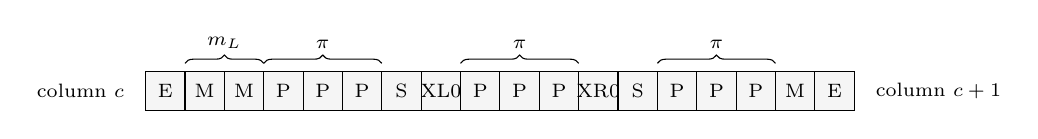
\begin{tikzpicture}[x=5mm,y=5mm,font=\scriptsize]
  \foreach \t [count=\i from 0] in {E,M,M,P,P,P,S,XL0,P,P,P,XR0,S,P,P,P,M,E} {
    \draw[fill=gray!8] (\i,0) rectangle ++(1,1);
    \node at (\i+0.5,0.5) {\t};
  }
  \draw[decorate,decoration={brace,amplitude=3pt}] (1,1.2) -- (3,1.2) node[midway,above=2pt] {$m_L$};
  \draw[decorate,decoration={brace,amplitude=3pt}] (3,1.2) -- (6,1.2) node[midway,above=2pt] {$\pi$};
  \draw[decorate,decoration={brace,amplitude=3pt}] (8,1.2) -- (11,1.2) node[midway,above=2pt] {$\pi$};
  \draw[decorate,decoration={brace,amplitude=3pt}] (13,1.2) -- (16,1.2) node[midway,above=2pt] {$\pi$};
  \node[anchor=east] at (-0.3,0.5) {column $c$};
  \node[anchor=west] at (18.3,0.5) {column $c+1$};
\end{tikzpicture}
\caption{The slots of a channel with one border level on each part, $m_L=2$, $m_R=1$, and a
pool of three tracks (before unused tracks are removed).}
\label{fig:pictorial-slots}
\end{figure}

\subsection{Maze search}\label{sec:pictorial-maze}

Each hop is routed by an A* search~\cite{hart1968formal} on the grid of a channel, in the
tradition of maze routing~\cite{lee1961algorithm}. Grid points are $(x, y)$ with $x$ a slot index
$0\le x<\mathit{width}$ and $y$ a half-lane between bounds $y_\text{lo}$ and $y_\text{hi}$. The
maze records: the set $H$ of used horizontal unit segments (keyed by their left point), the set
$V$ of used vertical unit segments (keyed by their upper point), the use of each point
(\code!e! end, \code!h! horizontal, \code!v! vertical, \code!x! crossing, \code!b! bend), a set of
blocked points, and the box rectangles $(\mathit{key}, x_0, x_1, y_t, y_b)$. The boxes containing
a point are cached. $\mathit{mid}$ is the mean of the first and last track slots.

\begin{algorithm}[Maze search]\label{alg:pictorial-maze}
Input: a start point leaving in direction $d_s$, a goal point entered in direction $d_g$, and a
flag \emph{relaxed}. Directions are $0:{+x}$, $1:{-x}$, $2:{+y}$, $3:{-y}$. Let
$\mathit{exits} = \mathrm{boxes}(\text{start})\setminus\mathrm{boxes}(\text{goal})$ and
$\mathit{enters} = \mathrm{boxes}(\text{goal})\setminus\mathrm{boxes}(\text{start})$. States are
(point, direction); the priority is cost plus Manhattan distance to the goal, ties broken by
cost, then by insertion count.
\begin{enumerate}
  \item Pop a state. If its point is the goal and it is not the start state, return the path.
    Skip a state whose recorded cost is lower.
  \item A point already in use (not the start, not relaxed) may only be passed straight through.
  \item For each direction $d'$: skip reversal, skip turning at a used point, and leave the start
    only in $d_s$. The next point must lie in the grid; reaching the goal requires $d'=d_g$; a
    non-goal point may not lie in an \code!E! slot; vertical moves are allowed only in
    \code!P! slots.
  \item The step costs 1, plus $\mathit{\_BEND} + 10^{-3}\,|x-\mathit{mid}|$ when $d'$ differs
    from the current direction.
  \item Unless relaxed: skip a used segment; skip a blocked point; at a point used by another
    wire, continue only when the point is not the goal and its use is perpendicular to the
    move (\code!v! for a horizontal move, \code!h! for a vertical one), adding
    $\mathit{\_CROSS}$; when the boxes containing the two points differ, the boxes left must lie
    in $\mathit{exits}$ and the boxes entered in $\mathit{enters}$.
  \item Relax the neighbor state when the new cost is lower.
\end{enumerate}
Return \py|None| when the queue empties.
\end{algorithm}

Taking a path marks its segments in $H$ or $V$, its two end points as \code!e!, a straight interior
point as \code!h! or \code!v! (or \code!x! when already used), and a turning point as \code!b!.
The result: no two wires share a segment or a bend, wires cross only at right angles, and a wire
crosses a box border only to enter or leave that box.

\subsection{Channel routing}\label{sec:pictorial-route}

\begin{algorithm}[Channel routing]\label{alg:pictorial-route}
Input: channel $\mathit{ch}$, its hops, and the lane span $(0, Y)$ with $Y$ the greatest band
bottom.
\begin{enumerate}
  \item Classify the boxes (\cref{def:pictorial-boxes}), compute the texts, the margins, the
    straight hops, the pool size $\pi$, and the border levels.
  \item Each hop's ends are (edge, lane): the left edge when the end's item lies in column
    $\mathit{ch}$, else the right edge. Order the hops by (not straight, $|l_a-l_b|$, index).
  \item Up to four attempts:
    \begin{enumerate}
      \item Build the slot types (\cref{def:pictorial-slots}).
      \item An inner box adds a rectangle over all slots and its lanes $[2t, 2b]$ and border
        lines at half-lanes $2t-1$ and $2b+1$ across the whole channel. A left box with border
        slot $x_b$ adds the rectangle $[0, x_b-1]$, border lines from 0 to $x_b$, and blocks its
        label row (points $(x, 2t)$ for $1\le x<x_b$). A right box adds the rectangle
        $[x_b+1, \mathit{width}-1]$ and border lines from $x_b$ to the right edge; a port-scoped
        right box also blocks its label row (points $(x,2t)$ for $x_b<x<\mathit{width}-1$). Every
        point of a border line is marked used \code!h!, and its segments enter $H$.
      \item The grid's half-lane bounds are $[-2, 2Y+2]$.
      \item Route the hops in order: from slot 0 (direction $+x$) or the last slot (direction
        $-x$) to slot 0 (entering in direction $-x$) or the last slot (entering in direction
        $+x$). On the last attempt, a failed strict search is repeated relaxed. Take every
        found path.
      \item When a hop finds no path, move it to the front of the order, double $\pi$, and try
        again.
    \end{enumerate}
  \item Keep every slot that is not a track, and every track slot used by a vertical segment
    or a bend; renumber the kept slots. Each path is reduced to its corner points (start, every
    turn, end).
\end{enumerate}
\end{algorithm}

\py|plan| routes the channels from $-1$ to $\mathit{columns}-1$ in order with the span
$(0, \max_k(\mathit{top}_k+\mathit{height}_k))$; a channel without hops is routed with an empty
hop list and keeps only its non-track slots. The \term{main lane} of a plan is the middle of the
lanes of component 0: $(\min \mathit{top} + \max(\mathit{top}+\mathit{height}-1))/2$ over its
items (0 when component 0 has no items); renderers put the diagram scalar on it.

\section{Labels}\label{sec:pictorial-labels}

\newcommand{\pgi}{\lstinline[style=pgrid,frame=none,basicstyle=\ttfamily]}

Every label is produced in one of three \term{label formats}: \code!tex! (matplotlib mathtext
without the enclosing dollar signs), \code!uni! (Unicode text), and \code!ascii!. The character
grid uses \code!uni! or \code!ascii!; the matplotlib figure uses \code!tex! and wraps each line
in dollar signs. Phases are stored in \emph{turns}, one turn being $2\pi$ (\cref{ch:algebra});
the engine notation prints turns, the publication notation prints radians.

\subsection{Expressions}\label{sec:pictorial-expr}

\begin{definition}[Cleaned expression]\label{def:pictorial-clean}
Before printing, an expression $e$ is \emph{cleaned}: an integer with $|e|>9999$ becomes the
unevaluated product of its prime powers in increasing prime order ($p^k$ for $k>1$, $p$ for
$k=1$); an expression containing a floating-point number is replaced by its SymPy
\py|nsimplify| rational form; any other expression is unchanged.
\end{definition}

\begin{algorithm}[Plain text]\label{alg:pictorial-text}
The plain text of $e$ is SymPy's \py|sstr| of the cleaned expression with every \code!**!
replaced by \code!^!. In format \code!ascii! that is the result. In format \code!uni! these
rewrites follow, in order:
\begin{enumerate}
  \item each whole-word Greek letter name (\code!alpha! \ldots\ \code!omega!, and the capitals
    \code!Gamma Delta Theta Lambda Xi Pi Sigma Upsilon Phi Psi Omega!) becomes its letter;
  \item \code!sqrt(w)! with a single word $w$ becomes \pgi!√w!, and any other \code!sqrt(!
    becomes \pgi!√(!;
  \item a whole-word \code!I! becomes \code!i!;
  \item a \code!*! is deleted when it follows a digit, \code!)!, or \pgi!π! and precedes a
    letter, \pgi!π!, a Greek letter, \pgi!√!, or \code!(!; a \code!*! after \pgi!π! is
    deleted;
  \item every remaining \code!*! becomes \pgi!·!.
\end{enumerate}
\end{algorithm}

\begin{algorithm}[Mathtext]\label{alg:pictorial-tex}
The mathtext of $e$ is SymPy's \py|latex| of the cleaned expression with
\py|mul_symbol="dot"|, then: \code!\cdot! after a digit, \code!\pi!, or a whole-word \code!i! is
deleted; \code!\cdot! before \code!\pi!, \code!e^!, a whole-word \code!i!, or \code!\sqrt! is
deleted; every remaining \code!" \cdot "! becomes \code!{\cdot}!.
\end{algorithm}

\subsection{Engine notation}\label{sec:pictorial-engine-labels}

In normal mode (\py|CONFIG.publication| false) a Z or X spider is labeled with its phase vector
as typed in the engine language (\cref{ch:language}). The label of every other generator is
empty, except that in format \code!tex! a triangle is labeled \code!T! and an inverse triangle
\code!T^{-1}!, in both modes.

\begin{definition}[Phase entries and family rule]\label{def:pictorial-entries}
For a spider with phase vector $\phi$ the \emph{entries} are the sparse nonzero entries
$\{k\mapsto\phi_k\}$ in turns, and the \emph{rule} is the family rule written in the printer's
index symbol (the first of \code!k!, \code!k1!, \code!k2!, \ldots\ not free in $\phi$) or none.
A concrete \emph{linear family} is detected and printed as a rule: when $\phi$ has no rule, its
dimension $r$ is concrete with $r>2$, it has more than one entry, and with $c = \phi_1$ every
difference $\phi_k - k c$ for $1\le k<r$ is an integer (zero modulo one turn), the entries become
empty and the rule becomes $c\cdot k$ with the integer symbol $k$.
\end{definition}

\begin{lstlisting}[style=grammar,caption={Engine label grammar (formats \texttt{uni} and \texttt{ascii}; the \texttt{tex} variants in brackets).}]
label   ::= ""                          -- no phase vector, or a zero one
          | phases                      -- unweighted
          | weights                     -- weighted, all phases zero
          | phases " MIDDOT " weights   -- [ "\ \cdot\ " ]
phases  ::= item { sep item } [ sep value " @k" ]       -- [ value "\,@k" ]
weights ::= "w: " item { sep item } [ sep value " @k" ] -- [ "w{:}\," ... ]
item    ::= value "@" index             -- index: decimal, increasing
sep     ::= ", "                        -- [ ",\ " ]
\end{lstlisting}
\code!MIDDOT! stands for the character U+00B7 (\pgi!·!), which appears in all three formats.
Values print in the label format (\cref{alg:pictorial-text,alg:pictorial-tex}); weights are the
explicit weight entries and the weight rule. The rule is always marked \code!@k!, whatever index
symbol the rule expression uses.

\subsection{Publication notation}\label{sec:pictorial-paper-labels}

In publication mode a Z or X spider is labeled in the notation of the qufinite ZXW
calculus~\cite{wang2023qufinitezxw,poor2023zxw}: the phase vector
$(\alpha_1,\dots,\alpha_{d-1})$ in radians, and for a weighted spider the coefficient vector
$(w_1 e^{i\alpha_1},\dots,w_{d-1}e^{i\alpha_{d-1}})$. A weighted spider is \term{boxed}: drawn
as a Z box or X box instead of a circle.

\begin{definition}[Radians]\label{def:pictorial-radians}
The radian form of a turns expression $t$ is
$\mathrm{simplify}\bigl(2\pi\cdot t[x\mapsto x/(2\pi)]\bigr)$, where the substitution runs over
every free symbol $x$ of $t$ not known to be an integer. A phase symbol such as $\alpha$ thus
reads as an angle already in radians, while integer symbols (dimensions, indices) stay in turns.
\end{definition}

\begin{algorithm}[Coefficient]\label{alg:pictorial-cis}
The coefficient text of weight $w$ and angle $\theta$ (both simplified) is the text of $w$ when
$\theta=0$. Otherwise let $\rho = \theta/\pi$. When $\rho$ contains no $\pi$ and is not a sum,
write $\rho = \mathit{num}/\mathit{den}$ and $\mathit{num} = c\cdot q$ with $c$ the numeric
coefficient; the exponent is the sign of $c$ (\code!-! or nothing), then $|c|$ unless it is 1,
then $\pi$, then \code!i!, then $q$ unless it is 1, then \code!/<den>! when
$\mathit{den}\neq1$. In format \code!ascii! the pieces are joined by \code!*! and $\pi$ prints
\code!pi*!; in format \code!uni! $\pi$ prints \pgi!π!; in format \code!tex! it prints
\code!\pi!. Otherwise the exponent is \code!i(<angle>)! for a sum and \code!i<angle>! for any
other $\theta$, with \code!<angle>! the text of $\theta$ (with a \code!*! after \code!i! in format \code!ascii!). The full text is
\code!<w>\,e^{<exponent>}! in format \code!tex!, \code!<w>MIDDOTe^(<exponent>)! in format
\code!uni!, and \code!<w>*exp(<exponent>)! in format \code!ascii!; the weight and its joiner are
omitted when $w=1$.
\end{algorithm}

\begin{algorithm}[Component vector]\label{alg:pictorial-vector}
Given the indices $I$ that carry entries, an optional family text $\mathit{fam}$, a flag
\emph{bare}, and a filler \emph{rest} (\code!0! for phases, \code!1! for coefficients), the
vector text is:
\begin{enumerate}
  \item $(\mathit{fam})_k$ when there is a family and $I=\emptyset$;
  \item at a concrete dimension $r$: the single value when $r=2$ and \emph{bare}, else
    $(v_1, \dots, v_{r-1})$;
  \item at a symbolic dimension with $I=\{1\}$ and no family: $v_1$ when \emph{bare}, else
    $(v_1)$;
  \item otherwise, with $m=\max I$ ($m=1$ when $I$ is empty): $(v_1,\dots,v_m, v_{m+1}, \dots)$
    with a family, or $(v_1,\dots,v_m, \mathit{rest}, \dots, \mathit{rest})$ without one.
\end{enumerate}
The ellipsis prints as \code!\dots!, \pgi!…!, or \code!...! in the three formats, and the
separator is that of the engine grammar.
\end{algorithm}

An unweighted spider prints the vector of its radian phases with \emph{bare} set, the family
being the radian form of the rule. A weighted spider prints the vector of coefficients
$w_k e^{i\alpha_k}$ (\cref{alg:pictorial-cis}) with \emph{bare} unset over the indices with a
phase entry or a weight entry; its family, when the phase or the weight has a rule, is the
coefficient of the weight rule (1 without one) and the radian phase rule (0 without one).

\begin{longtable}{@{}p{0.41\textwidth}p{0.18\textwidth}p{0.35\textwidth}@{}}
\caption{Spider labels in the two notations, as printed by the Unicode grid.}
\label{tab:pictorial-label-examples}\\
\toprule
Spider (engine language) & Normal & Publication \\
\midrule
\endfirsthead
\azx!Z(1 -> 1, literal 5) phase{1: 1/5, 2: 2/5, 3: 3/5, 4: 4/5}! & \pgi!k/5 @k! &
  \pgi!Ⓩ(2π/5, 4π/5, 6π/5, 8π/5)! \\
\azx!Z(1 -> 1) phase{1: alpha} weight{1: 2}! & \pgi!Ⓩα@1 · w: 2@1! & \pgi![Z](2·e^(iα))! \\
\azx!X(0 -> 1, literal 2) phase{1: 1/2}! & \pgi!Ⓧ1/2@1! & \pgi!Ⓧπ! \\
\azx!X(0 -> 1) phase{k: -k/d}! & \pgi!Ⓧ-k/d @k! & \pgi!Ⓧ(-2πk/d)_k! \\
\bottomrule
\end{longtable}

\subsection{Notes, dimensions, and scalars}\label{sec:pictorial-notes}

Below every drawing stand the \term{notes}, one per line, in this order:
\begin{enumerate}
  \item \code!phases in turns! -- in normal mode, when some Z or X item has a phase entry or a
    phase rule;
  \item \code!every wire has dimension <D>! -- when all wires share one dimension $D$ (in a
    figure $D$ is mathtext in dollar signs);
  \item \code!summarised: one box per term! -- in a summary;
  \item the view's own notes.
\end{enumerate}
Wire dimension labels are \emph{shown} exactly when the wires carry more than one distinct
dimension; then every wire is labeled once, in the margin of the channel of its first hop. A
\bbox{} always carries its multiplicity label. The diagram scalar is printed left of the
drawing, on the main lane, when it differs from 1; a large integer scalar prints in factored
form, so the scalar $123456$ prints \pgi!2^6·3·643! in Unicode.

\section{Character-Grid Renderer}\label{sec:pictorial-grid}

\py|grid(lay, unicode)| plans the layout with the grid metrics of \cref{tab:pictorial-metrics}
and paints a canvas of characters; it returns the rows joined by newlines, followed by the
notes.

\subsection{Cells}\label{sec:pictorial-cells}

The \term{cell} of an item is its text: the label of a boundary item, nothing for a dummy,
\code![<label>]! for a group, and for a node the glyph of \cref{tab:pictorial-glyphs} followed by
its label. A Z or X node prints \pgi!Ⓩ<label>! or \pgi!Ⓧ<label>! in Unicode and
\code!(Z <label>)! (\code!(Z)! without label) in ASCII; a boxed spider prints
\code![Z]<label>! or \code![X]<label>! in both. A shaded item with a nonempty cell gets a
trailing \code!*!.

\begin{longtable}{@{}p{0.08\textwidth}p{0.11\textwidth}p{0.11\textwidth}p{0.62\textwidth}@{}}
\caption{Glyphs per generator in the three renderers. $r$ is the spider radius and $h_b$ the
half box size (\cref{sec:pictorial-figure-geometry}); fg and bg are the ink and page
colors.}\label{tab:pictorial-glyphs}\\
\toprule
Kind & Unicode & ASCII & matplotlib \\
\midrule
\endfirsthead
\toprule
Kind & Unicode & ASCII & matplotlib \\
\midrule
\endhead
\code!Z! & \pgi!Ⓩ! & \code!(Z)! & circle of radius $r$, fill \code!#009e73!, edge fg; letter
  Z in \code!#111111! in normal mode; boxed: square of side $2h_b$, fill \code!#009e73! \\
\code!X! & \pgi!Ⓧ! & \code!(X)! & circle of radius $r$, fill \code!#cc3311!, edge fg; letter
  X in \code!#ffffff! in normal mode; boxed: square of side $2h_b$, fill \code!#cc3311! \\
\code!W! & \pgi!◀W! & \code!<W! & triangle filled with fg, apex left at $(x-h_b, y)$, flat
  side at $x+0.8h_b$ (snapped) \\
\code!F! & \pgi![F]! & \code![F]! & square of side $2h_b$, fill \code!#f2e07a!, letter F in
  \code!#111111! \\
\code!T! & \pgi!▷T! & \code!|>T! & triangle filled with bg, apex right at $(x+h_b,y)$, flat
  side at $x-0.8h_b$ (snapped); label $T$ above \\
\code!Ti! & \pgi!▶T⁻¹! & \code!|>T^-1! & the same triangle filled with \code!#b4b4b4!; label
  $T^{-1}$ above \\
\code!S! & \pgi!⊳S! & \code!>S! & trapezium, half height $h_b$ on the left and $0.5h_b$ on
  the right, fill \code!#c8c8c8!, letter S in \code!#111111! \\
\code!B! & \pgi!⊲B! & \code!<B! & trapezium, half height $0.5h_b$ on the left and $h_b$ on
  the right, fill \code!#c8c8c8!, letter B in \code!#111111! \\
\code!G! & \pgi!⏚! & \code!_|_! & earth symbol: a stem and three bars
  (\cref{sec:pictorial-figure-glyphs}) \\
group & \code![term ...]! & \code![term ...]! & rounded box with the term label \\
in, out & label & label & the label text \\
\bottomrule
\end{longtable}

\subsection{Columns and coordinates}\label{sec:pictorial-grid-coords}

\begin{algorithm}[Grid geometry]\label{alg:pictorial-grid-geometry}
\begin{enumerate}
  \item \emph{Brackets.} A non-boundary, non-dummy item needs a bracket on a side when that side
    has more than one port, or one port whose lane offset differs from the glyph lane. The glyph
    width $g_w$ of an item is its cell length plus its number of brackets.
  \item The width of column $c$ is the greatest $g_w$ of its items, at least 1. The scalar text
    (empty when the scalar is 1) reserves $\mathit{pad} = \mathrm{len}+2$ characters at the left
    (0 without scalar).
  \item \emph{Placement.} Starting at $x=\mathit{pad}$, for $c = -1, 0, \dots,
    \mathit{columns}-1$: column $c$ (when $c\ge0$) occupies its width, then channel $c$ occupies
    one character per slot.
  \item \emph{Frame growth}, up to three rounds while something grows: for each node-scoped
    \bbox{} with left border at $x_l$ and right border at $x_r$, let
    $\mathit{need} = \mathrm{len}(\mathit{mult})+1$ and
    $\mathit{short} = \max(\mathit{need} - (x_r - x_{\mathit{span}_1}),\ \mathit{need}+2-(x_r -
    x_l - 1))$, where $x_{\mathit{span}_1}$ is the start of the frame's last column; when
    positive, widen that column by $\mathit{short}$ and re-place.
  \item Lane $\lambda$ maps to row $2\lambda+1$; a half-lane $y$ maps to row $y+1$. An item's
    glyph starts at $x_\text{col} + \lfloor(\text{width}-g_w)/2\rfloor$ on the row of its glyph
    lane. A port attaches at the character right of the glyph (right side) or left of it (left
    side), on its lane's row; a dummy has no attachment.
\end{enumerate}
\end{algorithm}

\subsection{Painting}\label{sec:pictorial-paint}

\begin{algorithm}[Grid painting]\label{alg:pictorial-paint}
\begin{enumerate}
  \item \emph{Wires.} For each wire, collect its points: the start attachment, the corners of
    each hop mapped to (character, row), and the end attachment. Each axis-parallel segment
    marks every cell it covers with the direction bits $L, R, U, D$ toward its neighbors on the
    segment, per wire.
  \item A cell marked by two or more wires prints \pgi!┼! (ASCII \code!+!). A cell of one wire
    prints by its bits: $LR$ \pgi!─!, $UD$ \pgi!│!, $RD$ \pgi!┌!, $LD$ \pgi!┐!, $RU$ \pgi!└!,
    $LU$ \pgi!┘!, a lone horizontal bit \pgi!─!, a lone vertical bit \pgi!│!, anything else
    \pgi!─!; in ASCII \code!-!, \code!|!, \code!.!, \code!.!, \code!'!, \code!'!, \code!-!,
    \code!|!, and \code!-!.
  \item \emph{Frames.} A node-scoped \bbox{} with lanes $(t,b)$ is a rectangle from its left
    border character to its right border character, rows $2t$ to $2b+2$. A port-scoped
    \bbox{} runs from the port's attachment character to its border character in the adjacent
    channel, over the rows of its interior lanes plus one row above and below. Horizontal
    borders print \pgi!═! (\pgi!╪! where a wire passes), vertical borders \pgi!║! (\pgi!╫!
    where a wire passes), corners \pgi!╔!, \pgi!╗!, \pgi!╚!, \pgi!╝!; in ASCII \code!=!,
    \code!*!, \code!:!, \code!*!, and \code!#! for every corner. The character after the
    top-left corner is \code{!}, and the multiplicity label is right-aligned against the right
    border on the first interior row.
  \item \emph{Dimension labels.} When dimensions are shown, the label of each wire is centered in
    the margin of the channel of its first hop (the left margin when the hop starts at the left
    edge), on the hop's start row, provided the margin has room for it.
  \item \emph{Brackets.} For each bracketed side, a heavy bar spans the rows from the topmost to
    the bottommost of the side's port rows and the glyph row. On the right side the top, bottom,
    and middle port rows print \pgi!┎!, \pgi!┖!, \pgi!┠!; on the left side \pgi!┒!, \pgi!┚!,
    \pgi!┨!; rows without a port print \pgi!┃!. In ASCII the right side prints \code!]! and the
    left side \code![! throughout.
  \item \emph{Cells}, then the \emph{scalar} at column 0 of the row of the rounded main lane.
  \item Every row is stripped of trailing blanks; leading and trailing empty rows are removed;
    the notes follow.
\end{enumerate}
Texts (the \code{!} marks, multiplicity labels, and dimension labels) overwrite wires and
borders; brackets and cells overwrite everything.
\end{algorithm}

\section{Matplotlib Renderer}\label{sec:pictorial-figure}

\py|figure(lay, *, dark_theme, opaque=False, density=1, palette=None, fmt="png")| draws the
layout with matplotlib and returns the bytes of a PNG, PDF, or SVG file. For the duration of the
call it sets the matplotlib parameters \code!pdf.fonttype = 42! and
\code!svg.fonttype = "path"!, and in publication mode also \code!mathtext.fontset = "cm"!
(Computer Modern) and \code!font.family = "serif"!. The renderer imports matplotlib lazily;
matplotlib belongs to the optional dependency group \code!viz! of the package.

\subsection{Colors and sizes}\label{sec:pictorial-figure-geometry}

The ink and page colors $(\mathit{fg}, \mathit{bg})$ are \py|colours(dark_theme)|
(\cref{sec:pictorial-theme}); a \py|CONFIG.color| other than \code!auto! replaces $\mathit{fg}$;
a \py|palette| replaces both. With $s$ = \py|CONFIG.size| and
$\mathrm{snap}(v, n) = \max(n, n\cdot\mathrm{round}(72v/n))/72$ (a length in inches rounded to a
multiple of $n$ points, at least $n$ points), the geometry is:
\begin{center}
\begin{tabular}{@{}lll@{}}
\toprule
Quantity & Symbol & Value \\
\midrule
label font size & $f_\ell$ & $8.5s$ pt \\
letter font size & $f_g$ & $7.5s$ pt \\
dimension and note font size & $f_d$ & $0.85 f_\ell$ \\
scalar font size & & $1.1 f_\ell$ \\
slot width & $s_x$ & $\mathrm{snap}(0.085s, 2)$ in \\
lane pitch & $p_y$ & $\mathrm{snap}(0.22s, 2)$ in \\
spider radius & $r$ & $\mathrm{snap}(0.12s, 1)$ in \\
half box size & $h_b$ & $\mathrm{snap}(0.12s, 1)$ in \\
line width & & 1.0 pt \\
label line height & $h_\ell$ & $1.3 f_\ell/72$ in \\
\bottomrule
\end{tabular}
\end{center}
Lane $\lambda$ lies at height $Y(\lambda) = -\lambda p_y$; slot $i$ of a channel starting at $x$
has center $x + (i+0.5)s_x$. Text sizes are measured with matplotlib's \py|TextToPath| (as
mathtext when the text contains a dollar sign) and cached per (text, size).

\subsection{Label lines}\label{sec:pictorial-figure-labels}

The \code!tex! label of an item is split at every \code!,\ ! separator and refilled greedily:
a part joins the current line unless the line is nonempty and the joined line is wider than
$1.8s$ inches, in which case the current line ends with a comma and the part starts a new line.
Each line is wrapped in dollar signs. The item's label shrink factor is
$\min(1, \max(0.6, 2.2s/w))$ with $w$ the widest line. Label lines are centered horizontally on
the item and stacked in the item's label lanes: with $n$ lines, $\ell$ label lanes, and
$m = Y(\mathit{top} + (\ell-1)/2)$, line $j$ sits at height $m + (n-1-2j)h_\ell/2$, in size
$f_\ell$ times the shrink factor.

\subsection{Leg geometry}\label{sec:pictorial-legs}

Every port attaches through a two-point \term{leg}: an outline point on the glyph and a lane
point. With $\mathit{sgn} = +1$ on the right side and $-1$ on the left, port $j$ of $n$ on its
side, $\mathrm{spread}(n, j, h) = 0$ for $n=1$ and $h(1 - 2j/(n-1))$ otherwise, and $(x_0,y_0)$
the item center, \cref{tab:pictorial-legs} gives the outline point and the half width.

\begin{longtable}{@{}p{0.22\textwidth}p{0.50\textwidth}p{0.22\textwidth}@{}}
\caption{Outline points of the legs.}\label{tab:pictorial-legs}\\
\toprule
Glyph & Outline point & Half width \\
\midrule
\endfirsthead
Z, X circle & $(x_0+\mathit{sgn}\,r\cos\vartheta,\ y_0+r\sin\vartheta)$ with
  $\vartheta = \mathrm{spread}(n,j,55^\circ)$ & $r$ \\
in, out & $(x_0+\mathit{sgn}\cdot\mathit{half},\ y_0)$ & label width$/2 + 0.04s$ \\
W input & $(x_0-h_b,\ y_0)$ & $h_b$ \\
W outputs & $(\mathrm{snap}(x_0+0.8h_b),\ y_0+\mathrm{spread}(n,j,0.8h_b))$ & $h_b$ \\
T, Ti output & $(x_0+h_b,\ y_0)$ & $h_b$ \\
T, Ti inputs & $(\mathrm{snap}(x_0-0.8h_b),\ y_0+\mathrm{spread}(n,j,0.8h_b))$ & $h_b$ \\
S, B & $(x_0+\mathit{sgn}\,h_b,\ y_0+\mathrm{spread}(n,j,\sigma h_b))$ & $h_b$ \\
F, G, boxed spider, group & $(x_0+\mathit{sgn}\cdot\mathit{half},\
  y_0+\mathrm{spread}(n,j,0.7h_b))$ & $h_b$; a group: its width$/2$ \\
\bottomrule
\end{longtable}

For S and B, $\sigma = 0.4$ on the narrow side (the right side of S, the left side of B) and
$\sigma = 0.7$ on the wide side. The lane point is
\[
  \bigl(\mathrm{snap}\bigl(x_0 + \mathit{sgn}\,(\mathit{half} + 0.05s + 0.6\,|Y(\lambda_p) -
  y_\text{out}|)\bigr),\ Y(\lambda_p)\bigr),
\]
where $\lambda_p$ is the port's lane and $y_\text{out}$ the height of the outline point: a port
off its glyph's center reaches its lane by a slanted segment whose horizontal run grows with the
vertical offset.

\subsection{Canvas}\label{sec:pictorial-canvas}

\begin{algorithm}[Figure geometry]\label{alg:pictorial-figure-geometry}
\begin{enumerate}
  \item The shape width of an item is $2h_b$ for a boxed spider or any of F, T, Ti, W, S, B, G;
    $2r$ for an unboxed spider; the label width for a boundary item; the label width at
    $0.8f_\ell$ plus $0.12s$ for a group; 0 for a dummy.
  \item The width $w$ of column $c$ is the greatest of $\text{shape width}+0.14s$,
    $\text{label width}+0.08s$, and $2\cdot\text{reach}+0.06s$ over its items (the reach being
    the largest $|x|$ among the leg points computed with the item at $x_0=0$), then becomes
    $\mathrm{snap}(w + 1/72, 2)$.
  \item The scalar, when not 1, is \code!$<tex>$! with every \code!\frac! replaced by
    \code!\dfrac!; the left padding is $\mathrm{snap}(w_\text{scalar} + 0.25s + 0.15s)$, or
    $\mathrm{snap}(0.15s)$ without scalar.
  \item Placement runs as in the grid (column, then channel slots), followed by up to three
    rounds of frame growth with $\mathit{need}$ = multiplicity width at $f_\ell$ plus $0.1s$ and
    $\mathit{short} = \max(\mathit{need} - (x_r - x_{\mathit{span}_1}),\ \mathit{need}+0.25s -
    (x_r-x_l))$; a shortfall above $10^{-9}$ widens the last column by
    $\mathrm{snap}(\mathit{short}+1/72, 2)$.
  \item Each item's center is the middle of its column. The lane count is the greatest of the
    band bottoms, the node-scoped frame bottoms plus one, and the port-scoped frame bottoms plus
    one.
  \item With $n$ notes, the notes take $1.5\,n f_d/72 + 0.1s$ inches (0 without notes). The
    canvas spans from $y_\text{top} = Y(-1.5)$ down to
    $y_\text{bot} = Y(\text{lanes}+0.5) - \mathrm{snap}(\text{notes})$, and its width is
    $\mathrm{snap}(x_\text{end} + 0.15s)$, with $x_\text{end}$ the end of the last channel.
  \item The resolution is $\mathit{dpi} = 100\cdot\min\bigl(\mathit{density},\
    12000/(100\max(\text{width}, \text{height}))\bigr)$, so no side exceeds 12000 pixels.
  \item One axes fills the figure, without axis decoration; its limits are offset by half a
    point.
\end{enumerate}
\end{algorithm}

\subsection{Frames, wires, and labels}\label{sec:pictorial-figure-frames}

\paragraph{Frames.} A node-scoped \bbox{} is a dashed rectangle (dash pattern 4 on, 2 off,
line width 1, ink fg, no fill, drawing order 1) from its left border slot to its right border
slot, vertically from $Y(t)+p_y/2$ to $Y(b)-p_y/2$. A port-scoped \bbox{} on a right-side port
spans from the rightmost lane point of the item's right legs to its border slot (on a left-side
port, from its border slot to the leftmost lane point of the left legs), over its interior
lanes. Each frame shows \code{!} at $(x_l+0.05s,\ y_t-0.035s)$ in size $f_d$, anchored top left,
and its multiplicity at $(x_r - 0.06s,\ Y(t))$ in size $0.9f_\ell$, anchored right.

\paragraph{Wires.} A wire is one polyline: the start leg, the hop corners, and the end leg
reversed; ink fg, line width 1, mitre joins, butt caps, drawing order
$2+10^{-4}\cdot\mathit{index}$, and a halo (a stroke of width 3.4 in bg beneath it), so that a
crossing shows a gap in the lower wire. Where a wire segment crosses a frame border (a vertical
segment through a top or bottom edge strictly inside the frame's width, or a horizontal segment
through a side strictly inside its height), a dot marker of size $2.4s$ in fg marks the
crossing.

\paragraph{Dimension labels.} When dimensions are shown, each wire's label is centered on the
margin of its first hop's channel at the hop's start height, in size $f_d$, on a background box
in bg (padding 0.3), drawing order 5. A channel without margin slots shows no label.

\paragraph{Scalar and notes.} The scalar stands at $(0.15s, Y(\text{main lane}))$, anchored
left. Note $j$ (from 0) stands at $(0.1s,\ Y(\text{lanes}) - 0.05s - 1.5\,j f_d/72)$, anchored
top left, in size $f_d$.

\subsection{Node glyphs}\label{sec:pictorial-figure-glyphs}

Each non-dummy item draws its glyph (\cref{tab:pictorial-glyphs}) at its center $(x,y)$ in
drawing order 4, letters and labels in order 5:
\begin{itemize}
  \item A shaded item first draws a disc of radius $1.6\max(r,h_b)$ in fg at opacity 0.12; every
    artist the item draws after that disc gets opacity 0.55.
  \item A Z or X spider is a circle of radius $r$; in normal mode it carries its letter in size
    $0.85f_g$. A boxed spider is a square of side $2h_b$ without letter.
  \item W is the triangle with corners $(x-h_b,y)$ and $(\mathrm{snap}(x+0.8h_b), y\pm h_b)$,
    filled with fg. T and Ti are the triangles with corners $(\mathrm{snap}(x-0.8h_b), y\pm
    h_b)$ and $(x+h_b,y)$, filled with bg (T) or \code!#b4b4b4! (Ti).
  \item F is a square of side $2h_b$ with the letter F in size $f_g$.
  \item G, with $\mathit{sgn} = -1$ when the discard has an input port and $+1$ otherwise, is a
    stem from $x+\mathit{sgn}\,h_b$ to $x+0.4\,\mathit{sgn}\,h_b$ and three vertical bars at
    $x + \mathit{sgn}\cdot\{0.4, 0, -0.4\}h_b$ with half lengths $\{1, 0.62, 0.28\}h_b$, line
    width 1.6.
  \item S and B are the quadrilaterals with corners $(x-h_b, y\pm l)$ and $(x+h_b, y\pm q)$,
    where $(l, q) = (h_b, 0.5h_b)$ for S and $(0.5h_b, h_b)$ for B, with the letter in size
    $0.8f_g$.
  \item A group is a rounded box (pad 0.02) of the label's width and height $1.2h_b$, filled
    with bg, with the label in size $0.8f_\ell$.
  \item A boundary item prints its label in size $f_\ell$; a dollar sign in a label prints
    literally.
\end{itemize}

\paragraph{Saving.} The figure is saved in format \py|fmt| at the computed resolution, with a
transparent page unless \py|opaque| (then the page color is bg); the \code!fontTools! logger is
held at level \code!ERROR! while saving.

\section{Publication Mode}\label{sec:pictorial-publication}

The flag \py|CONFIG.publication| selects \term{publication mode}; normal mode is the default.
The shell sets it with the option \code!--publication!, the word \code!publication! (a toggle),
or the configuration key \code!publication! (\cref{sec:pictorial-config}). Publication mode
changes exactly these behaviors:
\begin{enumerate}
  \item spider labels use the publication notation (\cref{sec:pictorial-paper-labels}) instead
    of the engine notation;
  \item a weighted spider is boxed: \code![Z]! or \code![X]! in a grid, a filled square in a
    figure, with correspondingly wider glyph and leg geometry;
  \item the note \code!phases in turns! is omitted;
  \item a figure shows no letter inside a spider circle;
  \item a figure uses Computer Modern mathtext and serif text;
  \item the saved format \code!auto! means PDF instead of PNG (\cref{sec:pictorial-draw}).
\end{enumerate}
Layout, routing, colors, and every other glyph are identical in both modes.

\section{Rendering Dispatch and Saving}\label{sec:pictorial-draw}

\begin{signature}
\py|draw(view: View, style: str = "matplot") -> str|\\
\py|save_format() -> str|
\end{signature}

\py|save_format()| returns \py|CONFIG.format| unless it is \code!auto!, in which case it returns
\code!pdf! in publication mode and \code!png! otherwise.

\begin{algorithm}[Rendering dispatch]\label{alg:pictorial-draw}
\py|draw(view, style)|:
\begin{enumerate}
  \item Raise \py|ValueError("unknown drawing style '<style>'")| (the style in Python
    \py|repr| form) when \py|style| is not in \py|STYLES|.
  \item $\mathit{lay}\gets$ \py|layout(view)|. The protocol $P$ is \py|protocol()| for style
    \code!matplot! and \code!none! for the other styles.
  \item If $P\neq$ \code!none! or a save folder is set:
    \begin{enumerate}
      \item the display density is $\mathit{dense} = $ \py|density(lay)| when $P$ is \code!none!
        or scalable (\cref{sec:pictorial-encodings}), else 1;
      \item if a save folder is set: with \py|SAVE_WHITE|, render
        \py|figure(lay, dark_theme=False, opaque=True, density=density(lay), palette=WHITE, fmt=ext)|;
        otherwise render \py|figure(lay, dark_theme=dark(), opaque=True, density=dense, fmt=ext)|,
        with $\mathit{ext}$ = \py|save_format()|. Write the bytes with
        \py|keep(data, "zx", ext)|. A PNG rendered without \py|SAVE_WHITE| doubles as the
        display image;
      \item if $P\neq$ \code!none! and no display image exists yet, render
        \py|figure(lay, dark_theme=dark(), opaque=(P == "sixel"), density=dense)| as PNG;
      \item any exception in these renders discards the display image;
      \item with a display image and style \code!matplot!, return
        \py|encode_image(png, P, dense)| when it is not \py|None|.
    \end{enumerate}
  \item Fall back to text: style \code!matplot! becomes \code!unicode!, and \code!unicode!
    becomes \code!ascii! when the encoding of standard output, lowercased with hyphens removed,
    is neither \code!utf8! nor \code!utf8sig! (a missing encoding counts as neither). Return
    \py|grid(lay, unicode=(style == "unicode"))|.
\end{enumerate}
\end{algorithm}

A save folder thus receives one file per drawn diagram in every style, including
\code!unicode! and \code!ascii!: the text style decides the screen output, while the file is
always the matplotlib drawing. Without matplotlib (or with any rendering error) the screen shows
the character grid and no file is written.

\section{Sizing}\label{sec:pictorial-sizing}

A rendered image has two sizes: its pixel size and its displayed size on the terminal. The
\term{density} is the number of rendered pixels per displayed pixel.

\begin{definition}[Drawing density]\label{def:pictorial-density}
With $N$ the number of non-dummy items of the layout,
\[
  \mathit{density} = \min\Bigl(8,\ 2\max\bigl(1, \sqrt{N/40}\bigr)\cdot \kappa\Bigr),\qquad
  \kappa = \max\Bigl(1,\ \frac{(1.6\,C + 2)\cdot0.9\cdot s\cdot100}{\max(10,\ W-1)\cdot w_c}\Bigr),
\]
where $C$ is the number of columns, $s$ = \py|CONFIG.size|, $W$ the terminal width in columns
(from \py|shutil.get_terminal_size|), and $w_c$ the character cell width in pixels;
$\kappa = 1$ when the cell width is unknown. The numerator estimates the figure's natural width
in pixels at 100 dpi; a figure wider than the terminal is rendered denser so that it keeps its
detail when shown scaled down.
\end{definition}

The figure resolution is $100\cdot\min(\mathit{density}, 12000/(100\cdot\text{longest side in
inches}))$ dots per inch (\cref{alg:pictorial-figure-geometry}), and the mathtext resolution is
$100\cdot\min(\mathit{density}, 12000/\text{longest side in pixels})$
(\cref{sec:pictorial-mathtext}); neither image has a side longer than
\py|_MAX_PIXELS| $= 12000$ pixels.

\begin{definition}[Display cells]\label{def:pictorial-cells}
\py|cells(png, density)| returns \py|None| unless the terminal's cell height and width are both
known and the PNG has at least 24 bytes. Otherwise it reads the width $w$ and height $h$ from the
PNG header (big-endian 32-bit integers at bytes 16--19 and 20--23), computes
$c = w/(\mathit{density}\cdot w_c)$ columns and $r = h/(\mathit{density}\cdot h_c)$ rows, caps
$c$ at $\mathit{room} = \max(10, W-1)$ keeping the aspect ratio ($r \gets r\cdot\mathit{room}/c$,
$c\gets\mathit{room}$), and returns $(\max(1,\lceil c\rceil), \max(1,\lceil r\rceil))$.
\end{definition}

\section{Terminal}\label{sec:pictorial-terminal}

\module{archytaszx.repl.terminal} holds the terminal facts, the display settings, the save
folder, the mathtext renderer, and the image encoders. Its environment variables are listed in
\cref{tab:pictorial-env}; every function that reads the environment accepts an optional mapping
\py|environ| in place of \py|os.environ|.

\begin{longtable}{@{}p{0.30\textwidth}p{0.64\textwidth}@{}}
\caption{Environment variables read by the terminal module.}\label{tab:pictorial-env}\\
\toprule
Variable & Effect \\
\midrule
\endfirsthead
\code!ARCHYTASZX_IMAGES! & Forces the image protocol when its lowercased value is one of
  \code!kitty!, \code!iterm!, \code!sixel!, \code!none!. \\
\code!ARCHYTASZX_IMAGE_THEME! & \code!dark! or \code!light! (lowercased) fixes the theme. \\
\code!ARCHYTASZX_IMAGE_FG! & Ink color of images, before the terminal's reported color. \\
\code!COLORFGBG! & The text after its last \code!;! is the background color number; 7 or 15
  means a light theme. \\
\code!TERM!, \code!TERM_PROGRAM!, \code!KITTY_WINDOW_ID!, \code!LC_TERMINAL! & Protocol
  detection (\cref{alg:pictorial-protocol}). \\
\code!XDG_CONFIG_HOME! & Base folder of the configuration file. \\
\bottomrule
\end{longtable}

\subsection{Image protocol detection}\label{sec:pictorial-protocol}

\begin{algorithm}[Protocol detection]\label{alg:pictorial-protocol}
\py|protocol(environ=None, tty=None)|:
\begin{enumerate}
  \item If \code!ARCHYTASZX_IMAGES!, lowercased, is in \py|PROTOCOLS|, return it.
  \item If standard output is not a terminal (\py|sys.stdout.isatty()|, or the \py|tty|
    argument when given), return \code!none!.
  \item Return \code!kitty! when \code!KITTY_WINDOW_ID! is set, \code!TERM! is
    \code!xterm-kitty! or \code!xterm-ghostty!, or \code!TERM_PROGRAM! is \code!ghostty!.
  \item Return \code!iterm! when \code!TERM_PROGRAM! is \code!iTerm.app!, \code!WezTerm!, or
    \code!vscode!, or \code!LC_TERMINAL! is \code!iTerm2!.
  \item Return \code!sixel! when \code!TERM! contains \code!sixel!, starts with \code!foot! or
    \code!mlterm!, or \code!TERM_PROGRAM! is \code!mlterm!.
  \item Return \code!none!.
\end{enumerate}
\end{algorithm}

\subsection{Theme and colors}\label{sec:pictorial-theme}

\py|dark(environ=None)| returns \py|True| or \py|False| from \code!ARCHYTASZX_IMAGE_THEME! when
it is \code!dark! or \code!light!; otherwise it takes the part of \code!COLORFGBG! after the last
semicolon and returns \py|False| exactly when that part is the decimal number 7 or 15. A missing
or unparsable \code!COLORFGBG! means a dark theme.

\py|colours(dark_theme, environ=None)| returns $(\mathit{fg}, \mathit{bg})$: the foreground is
the first nonempty value among \code!ARCHYTASZX_IMAGE_FG!, \py|TERMINAL.fg|, and the theme
default; the background is \py|TERMINAL.bg| when known, else the theme default. The theme
defaults are ink \code!#e6e6e6! on \code!#1e1e1e! for a dark theme and ink \code!#111111! on
\code!#ffffff! for a light one. Both renderers then let a
\py|CONFIG.color| other than \code!auto! replace $\mathit{fg}$, and an explicit palette replace
both.

\subsection{Terminal queries}\label{sec:pictorial-queries}

\begin{definition}[Terminal facts]\label{def:pictorial-terminal}
\py|Terminal(fg, bg, cell, cell_width)| records the foreground and background colors as
\code!#rrggbb! and the character cell height and width in pixels, each \py|None| when unknown.
The module value \py|TERMINAL| starts as \py|Terminal()| (all unknown) and is replaced by
\py|prepare|.
\end{definition}

\begin{algorithm}[Terminal query]\label{alg:pictorial-query}
\py|query_terminal()|:
\begin{enumerate}
  \item Open \file{/dev/tty} for reading and writing without making it the controlling
    terminal; on \py|ImportError| (no \py|termios|) or \py|OSError| return \py|Terminal()|.
  \item Save the terminal attributes and switch to cbreak mode.
  \item Send three requests, each answered within 0.2 seconds or ignored:
    \begin{itemize}
      \item foreground color, OSC 10: \code!ESC ] 1 0 ; ? ESC \! (the bytes
        \code!\x1b]10;?\x1b\\!), reply matched by \code!ESC]10;rgb:R/G/B!;
      \item background color, OSC 11: \code!\x1b]11;?\x1b\\!, reply
        \code!ESC]11;rgb:R/G/B!;
      \item cell size in pixels, CSI 16 t: \code!\x1b[16t!, reply \code!ESC[6;H;Wt!.
    \end{itemize}
    The reply is read in chunks of up to 256 bytes (decoded as UTF-8 with replacement) until the
    pattern matches or the 0.2-second deadline passes.
  \item Restore the attributes (flushing pending input) and close the descriptor; a
    \py|termios.error| or \py|OSError| during the exchange returns \py|Terminal()|.
  \item Each color component of $n$ hexadecimal digits becomes the two-digit hexadecimal of
    $\lfloor v\cdot255/(16^n-1)\rfloor$; the color is \code!#! followed by the three
    components. The cell height $H$ and width $W$ are kept when positive.
\end{enumerate}
\end{algorithm}

\py|prepare(environ=None)| does nothing when \py|protocol(environ)| is \code!none!. Otherwise it
replaces \py|TERMINAL| with \py|query_terminal()| when both standard input and standard output
are terminals, and, once per process, starts a daemon thread that renders the mathtext line
\code!\sum_{x=0}^{q-1} |x\rangle! with a dark theme, which imports and initializes matplotlib
in the background. The shell calls \py|prepare| at start-up when the initial notation mode is not
DIRAC and the initial style is \code!matplot! (\cref{sec:pictorial-integration}).

\subsection{Display settings}\label{sec:pictorial-config}

\begin{definition}[Display settings]\label{def:pictorial-config}
\py|Config(size=1.0, color="auto", format="auto", publication=False)|:
\py|size| scales all text and geometry (1 means the terminal's cell height for mathtext and the
sizes of \cref{sec:pictorial-figure-geometry} for figures); \py|color| is \code!auto! (the
terminal's text color) or a color; \py|format| is the saved drawing format; \py|publication|
selects publication mode. The module value \py|CONFIG| holds the settings in use.
\end{definition}

\py|set_config(config, key, value)| sets one setting and raises \py|ValueError| with these exact
messages:
\begin{itemize}
  \item \code!size!: the value converted with \py|float|; on failure
    \code!size must be a number, got <repr>!; outside $(0, 10]$
    \code!size must be in (0, 10]!.
  \item \code!color!: the value as stripped text; accepted when it is \code!auto!, matches
    \code!#! followed by exactly 3 or 6 hexadecimal digits, or is a color name that matplotlib
    accepts (\py|matplotlib.colors.is_color_like|; no names without matplotlib); otherwise
    \code!color must be auto, #rgb, #rrggbb or a colour name, got <repr>!.
  \item \code!format!: the stripped, lowercased text, one of \py|FORMATS|; otherwise
    \code!format must be one of auto, png, pdf, svg, got <repr>!.
  \item \code!publication!: a Boolean, or text whose stripped lowercase form is \code!true!,
    \code!on!, \code!yes!, \code!1! (true) or \code!false!, \code!off!, \code!no!, \code!0!
    (false); otherwise \code!publication must be true or false, got <repr>!.
  \item any other key: \code!unknown setting <repr>; settings: size, color, format, publication!.
\end{itemize}

\paragraph{Configuration file.} \py|config_path(environ=None)| is
\file{$XDG_CONFIG_HOME/archytaszx/config.toml}, with \file{~/.config} in place of
\code!$XDG_CONFIG_HOME! when that variable is unset or empty. \py|load_config(path=None)| reads
the \tool{TOML}{https://toml.io/en/v1.0.0} file at the path (default \py|config_path()|) and
applies every top-level key with \py|set_config|; a missing file gives the defaults; an
unreadable or malformed file raises \py|ValueError("cannot read <path>: <error>")|.
\py|save_config(config, path=None)| creates the folder and writes exactly four lines, then
returns the path:
\begin{lstlisting}[style=grammar]
size = <Python repr of the float, e.g. 1.0>
color = "<color>"
format = "<format>"
publication = <true|false>
\end{lstlisting}

The shell reads the file at start-up into \py|CONFIG|; on \py|ValueError| it writes
\code!archytaszx: <message>; using the default display settings! to standard error. The shell
word \code!config! prints the settings as
\begin{lstlisting}[style=grammar]
size = <size, Python format g>
color = <color>
format = <format>
publication = <true|false>
file: <config path>
\end{lstlisting}
\code!config KEY VALUE! sets one setting (the key lowercased), \code!config save! writes the file
and prints \code!saved <path>!, \code!config reset! restores the defaults, and any other argument
is the error \code!usage: config [KEY VALUE | save | reset]!; an error prints
\code!error: <message>! and counts as a failed line.

\subsection{Mathtext images}\label{sec:pictorial-mathtext}

\begin{signature}
\py|render_png(lines: list[str], *, dark_theme: bool, opaque: bool = False, density: float = 1, palette: tuple[str, str] | None = None) -> bytes|
\end{signature}

\py|render_png| draws each line as matplotlib mathtext (the stripped line wrapped in dollar
signs) and returns a PNG. When the warm-up thread exists and the caller is another thread, it
first waits for the warm-up to finish.
\begin{enumerate}
  \item Colors: \py|colours(dark_theme)|, then \py|CONFIG.color|, then \py|palette|, as for
    figures.
  \item The text height is $\mathit{px} = (0.75\,h_c \text{ when the cell height } h_c
    \text{ is known, else } 14)\cdot s$ pixels; the font size is $72\,\mathit{px}/100$ points.
  \item Each line is placed left-aligned with vertical alignment at its bottom; its extent is
    measured with the Agg renderer. The padding and the gap between lines are both
    $\mathit{px}/3$. The image is $\max(\text{line width}) + 2\,\mathit{pad}$ wide and
    $\sum\text{line height} + \mathit{gap}\,(n-1) + 2\,\mathit{pad}$ high, at 100 dpi.
  \item Lines are stacked from the top: each line's bottom sits at the running height, which
    then drops by the line height and the gap.
  \item The PNG is saved at $100\min(\mathit{density}, 12000/\max(\text{width},
    \text{height}))$ dpi, transparent unless \py|opaque|.
\end{enumerate}
The current code calls \py|render_png| only from the warm-up thread; no command shows Dirac
notation or any other text as an image.

\subsection{Image encodings}\label{sec:pictorial-encodings}

\begin{signature}
\py|encode_image(png: bytes, proto: str | None = None, density: float = 1) -> str | None|\\
\py|scalable(proto: str) -> bool|
\end{signature}

\py|encode_image| returns \py|None| for protocol \code!none! (the default protocol is
\py|protocol()|). For \code!kitty! and \code!iterm! it computes the display size
\py|cells(png, density)| (\cref{def:pictorial-cells}), which may be \py|None|; sixel ignores the
size. \py|scalable(proto)| is true for \code!iterm!, and for \code!kitty! when the cell width is
known: these protocols can show an image smaller than its pixel size, so \py|draw| renders them
at the full density. On the other protocols \py|draw| renders at density 1.

\begin{lstlisting}[style=grammar,caption={Inline-image escape sequences. ESC is byte 0x1B, BEL is 0x07, and ST is the two bytes ESC backslash.}]
kitty  ::= first { more }
first  ::= ESC "_G" "a=T,f=100" [ ",c=" cols ",r=" rows ] ",m=" flag ";" chunk ST
more   ::= ESC "_G" "m=" flag ";" chunk ST
chunk  ::= up to 4096 characters of the standard base64 text of the PNG
flag   ::= "1"   -- more chunks follow
         | "0"   -- last chunk

iterm  ::= ESC "]1337;File=inline=1;size=" bytes [ fit ]
           ";preserveAspectRatio=1:" base64 BEL
fit    ::= ";width=" cols ";height=" rows          -- when cells() is known
         | ";width=" pw "px;height=" ph "px"       -- else, when density != 1

sixel  ::= ESC "Pq" '"1;1;' width ";" height palette band { "-" band } ST
palette::= { "#" c ";2;" p ";" p ";" p }           -- c = 0..15, p = round(100*c/15)
band   ::= colour { "$" colour }
colour ::= "#" c { run }
run    ::= "!" n char                              -- n > 3 repeats
         | char { char }                           -- up to 3 repeats written out
\end{lstlisting}

\paragraph{Kitty.} The PNG (\code!f=100!) is transmitted and displayed at once (\code!a=T!) in
chunks of 4096 base64 characters; an empty PNG gives one empty chunk. The first chunk carries
the display size in cells when known
(\tool{kitty graphics protocol}{https://sw.kovidgoyal.net/kitty/graphics-protocol/}).

\paragraph{iTerm2.} The image is one OSC 1337 \code!File! sequence with the byte length of the
PNG. With known cells the width and height are in cells; otherwise, when $\mathit{density}\neq1$
and the PNG has a header, they are $\mathrm{round}(w/\mathit{density})$ and
$\mathrm{round}(h/\mathit{density})$ pixels; otherwise there is no size.

\paragraph{Sixel.} The PNG is decoded to RGBA floats in $[0,1]$; each pixel's gray value is the
mean of its red, green, and blue components (alpha is ignored), quantized to
$c = \mathrm{round}(15\cdot\mathit{grey})$. The palette defines 16 gray levels in the RGB
percentage form. The image is cut into bands of 6 rows. Within a band, for each gray level
present (in increasing order), each pixel column becomes the character
$\mathrm{chr}(63 + \sum_{i} 2^i [\text{row } i \text{ has level } c])$, and runs of equal
characters longer than 3 are compressed to \code!!<n><char>!. The levels of one band are
separated by \code!$! (carriage return) and the bands by \code!-! (line feed). The raster
attributes \code!"1;1;W;H! declare a pixel aspect ratio of 1:1 and the image size. The display
size cannot be scaled, which is why \py|draw| renders sixel images opaque at density 1.

\subsection{Saved images}\label{sec:pictorial-saved}

\py|SAVE_DIR| (default \py|None|) is the folder that receives every rendered drawing, and
\py|SAVE_WHITE| (default \py|False|) makes saved drawings black on white (palette
\py|WHITE|, that is \code!#000000! on \code!#ffffff!, opaque, at \py|density(lay)|).
\py|keep(data, kind, ext="png")| returns \py|None| without a folder; otherwise it creates the folder, increments
a per-process counter starting at 1, writes the bytes to \file{<SAVE_DIR>/NNNN-<kind>.<ext>} with
the counter as four zero-padded digits, and returns the path. \py|draw| uses the kind \code!zx!,
so a session's drawings are \file{0001-zx.png}, \file{0002-zx.png}, and so on. The shell options
\code!--images DIR! and \code!--images_white DIR! (mutually exclusive) set \py|SAVE_DIR| to
\code!DIR!, the second also setting \py|SAVE_WHITE|.

\section{Integration with the Printer and the Shell}\label{sec:pictorial-integration}

\paragraph{Drawing hook.} The printer keeps a context variable holding an optional function
from \py|Diagram| to \py|str| (default \py|None|). \py|drawing(draw)| sets it for the duration of
a \py|with| block and restores the previous value afterward. In notation mode ZX a diagram
renders as \py|draw(diagram)|, or as its graph listing when no function is set; in BOTH it
renders as the same block followed by the Dirac block; RAW always renders the graph listing and
DIRAC never draws. A scalable diagram (\cref{ch:diagrams}) is converted with
\py|from_scalable| and drawn; when the conversion fails, or no function is set, its scalable
graph listing appears instead. Every diagram inside a composite state is rendered through the
same dispatch: the result of a rewrite, every state of a derivation and of a certificate (each
state recovered by replaying the steps), both halves of a proof certificate, and the states of an
induction proof. Each such block is indented by the printer's listing indent, which then also
precedes any image escape sequence.

\paragraph{Outcome formatting.}
\py|commands.format_outcome(outcome, mode, *, unicode, zx_style="matplot", listing=False, doubled=False)|
installs the drawing hook in modes ZX and BOTH
with a function that, for each diagram:
\begin{enumerate}
  \item builds \py|View(diagram)|; with \py|doubled| and a diagram that is not pure, builds the
    doubled diagram (\cref{ch:mixed}) instead and shades every node whose origin lies on the
    conjugate sheet;
  \item draws it with \py|draw(view, zx_style)|;
  \item with \py|listing|, appends a newline and the graph listing of the original diagram.
\end{enumerate}
An unknown \py|zx_style| raises \py|CommandGrammarError("unknown ZX drawing style <repr>")|; a
rendering exception within one block prints
\code!render: unavailable (<exception type>: <message>)! in its place.

\paragraph{Shell words and options.} \Cref{tab:pictorial-views} lists the view words. Each word,
typed alone (optionally after a colon), sets the notation mode and, when the word names one, the
drawing style, and prints \code!mode: <word>!; the same words with two leading dashes or one are
mutually exclusive command-line options (default \code!--dirac!). The words \code!listing!,
\code!doubled!, and \code!publication! toggle their flags and print \code!listing: on! or
\code!listing: off! (and likewise). The interactive loop calls \py|prepare| at start-up when the
mode is not DIRAC and the style is \code!matplot!, and the script runner (\code!-c! commands or
script files) does the same before running; switching to a drawing mode later with a view word
does not call \py|prepare|, so the terminal facts then stay unknown.

\begin{longtable}{@{}p{0.16\textwidth}p{0.14\textwidth}p{0.14\textwidth}p{0.48\textwidth}@{}}
\caption{View words of the shell.}\label{tab:pictorial-views}\\
\toprule
Word & Mode & Style & Help text \\
\midrule
\endfirsthead
\code!dirac! & DIRAC & unchanged & show Dirac notation \\
\code!zx! & ZX & \code!matplot! & draw ZX diagrams with matplotlib (alias of
  \code!--zxrender!) \\
\code!zxrender! & ZX & \code!matplot! & draw ZX diagrams with matplotlib, Unicode without an
  image protocol \\
\code!zxunicode! & ZX & \code!unicode! & draw ZX diagrams on a Unicode character grid \\
\code!zxascii! & ZX & \code!ascii! & draw ZX diagrams on an ASCII character grid \\
\code!both! & BOTH & \code!matplot! & show Dirac notation and the matplotlib ZX drawing \\
\code!raw! & RAW & unchanged & print full ZX graph listings, nothing summarized or capped \\
\bottomrule
\end{longtable}

\paragraph{Python embedding.} The embedding (\cref{ch:python-api}) draws through the same code:
a network's \py|draw(style="unicode")| returns \py|draw(View(diagram), style)|, and its
\py|_repr_png_()| (the rich display hook of \tool{Jupyter}{https://jupyter.org}) returns
\py|figure(layout(View(diagram)), dark_theme=False, opaque=True, palette=WHITE)|: a PNG, black on
white, at density 1.

\section{Worked Examples}\label{sec:pictorial-examples}

The figures of this section are the output of
\py|figure(..., palette=WHITE, opaque=True, fmt="pdf")| for the stated diagrams, in normal and in publication mode, and the listings are
the output of \py|grid| for the same layouts, copied verbatim.

\subsection{GHZ state with a port-scoped !-box}\label{sec:pictorial-ex-ghz}

The symbolic GHZ state~\cite{ghz1989beyond} on $n+1$ qudits of dimension $d$ is a Z spider with
one plain output and one output repeated by a port-scoped \bbox{} of multiplicity $n$, with
scalar $d^{-1/2}$:
\begin{lstlisting}[style=azx]
load
  count n
  g = Z(0 -> 2)
  repeat n: g.out1
  scalar d^(-1/2)
\end{lstlisting}

\begin{figure}[ht]
\centering
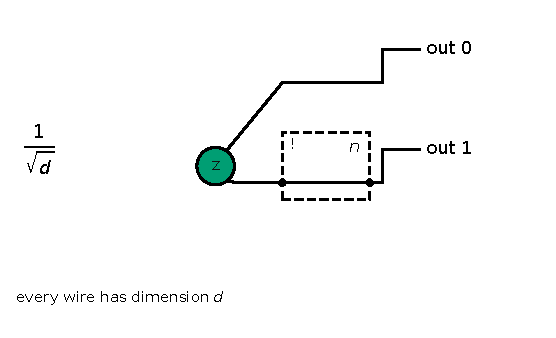
\includegraphics[width=0.45\textwidth]{figures/pictorial-ghz.pdf}\hfill
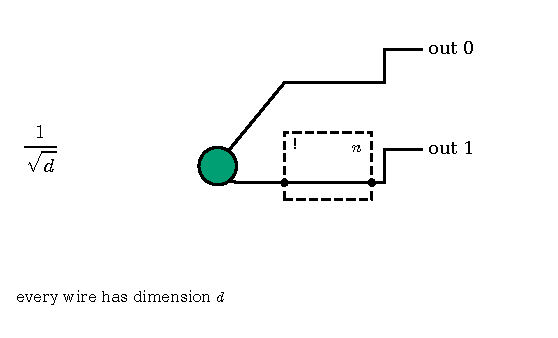
\includegraphics[width=0.45\textwidth]{figures/pictorial-ghz-pub.pdf}
\caption{The GHZ state in normal mode (left) and publication mode (right). The port-scoped
\texorpdfstring{!-box}{!-box} frames the repeated output; dots mark where the wire crosses its border.}
\label{fig:pictorial-ghz}
\end{figure}

The Z spider has two right-side ports, so its band is two lanes high and the grid draws a heavy
bracket on its right. The port-scoped \bbox{} adds one label lane above and one padding lane
below the repeated port (\cref{alg:pictorial-bands}), which pushes the plain output to lane 0.
All wires share dimension $d$, so no wire is labeled and the note says so.
\begin{lstlisting}[style=pgrid]
                  ┌──out 0
                  │
           ┎──────┘
           ┃╔!═══╗
1/√d      Ⓩ┃║   n║┌──out 1
           ┃║    ║│
           ┖╫────╫┘
            ╚════╝
every wire has dimension d
\end{lstlisting}
\begin{lstlisting}[style=pgrid]
                         .--out 0
                         |
                  ]------'
                  ]#!===#
1/sqrt(d)      (Z)]:   n:.--out 1
                  ]:    :|
                  ]*----*'
                   #====#
every wire has dimension d
\end{lstlisting}

\subsection{GHZ preparation with a node-scoped !-box}\label{sec:pictorial-ex-circuit}

The preparation circuit of the same state applies an X state, a Fourier box, and a Z spider,
then $n$ controlled additions, each an X spider fed by a fresh X state, inside a node-scoped
\bbox:
\begin{lstlisting}[style=azx]
load
  count n
  X(0 -> 1) -> F -> z = Z(1 -> 2)
  repeat n: z.out1 -> t = X(2 -> 1), X(0 -> 1) -> t
  scalar d^(-1/2)
\end{lstlisting}

\begin{figure}[ht]
\centering
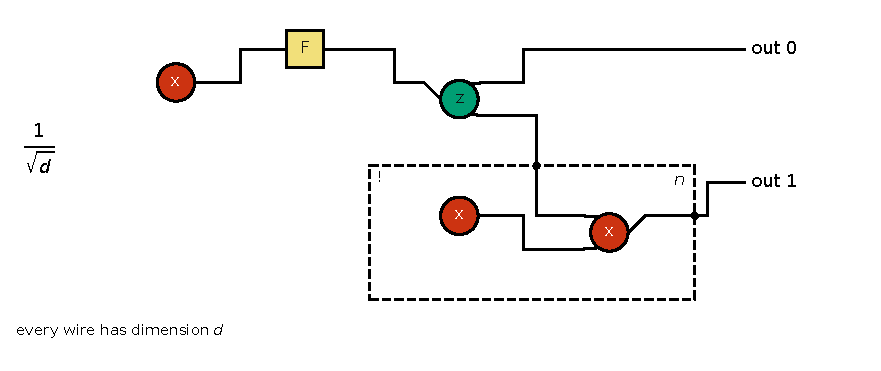
\includegraphics[width=0.75\textwidth]{figures/pictorial-ghzcircuit.pdf}\\[2mm]
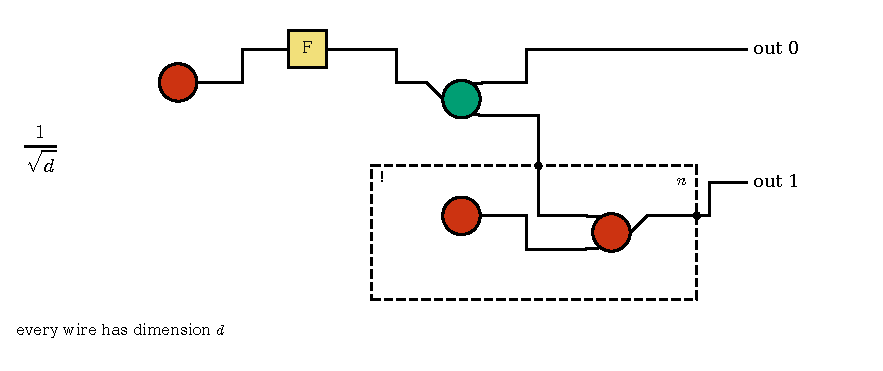
\includegraphics[width=0.75\textwidth]{figures/pictorial-ghzcircuit-pub.pdf}
\caption{GHZ preparation in normal mode (top) and publication mode (bottom). The node-scoped
\texorpdfstring{!-box}{!-box} holds both X spiders of the repeated step and spans two columns.}
\label{fig:pictorial-ghzcircuit}
\end{figure}

Layer assignment puts the X state in column 0 (it is a source with no input, so it is pulled
right next to F), F in column 1, Z in column 2, the inner X state and the X spider in columns 3
and 4, and both outputs in column 5. The wire from Z to the inner X spider enters the frame from
above, crossing its top border at a right angle (\pgi!╪! in the grid, a dot in the figure).
\begin{lstlisting}[style=pgrid]
             ┌──[F]────┐      ┌─────────┐
             │         │      │         │
          Ⓧ──┘         └──Ⓩ┎──┘         └──out 0
                           ┃
                           ┖───┐
                               │
                               │
                     ╔!════════╪═══════╗
1/√d                 ║         │      n║┌──out 1
                     ║         │       ║│
                     ║    Ⓧ───┐│       ║│
                     ║        ││       ║│
                     ║        │└──┒Ⓧ───╫┘
                     ║        │   ┃    ║
                     ║        └───┚    ║
                     ║                 ║
                     ║                 ║
                     ╚═════════════════╝
every wire has dimension d
\end{lstlisting}
\begin{lstlisting}[style=pgrid]
                    .--[F]----.        .-----------.
                    |         |        |           |
               (X)--'         '--(Z)]--'           '--out 0
                                    ]
                                    ]---.
                                        |
                                        |
                            #!==========*=========#
1/sqrt(d)                   :           |        n:.--out 1
                            :           |         :|
                            :    (X)---.|         :|
                            :          ||         :|
                            :          |'--[(X)---*'
                            :          |   ]      :
                            :          '---[      :
                            :                     :
                            :                     :
                            #=====================#
every wire has dimension d
\end{lstlisting}

\begin{figure}[ht]
\centering
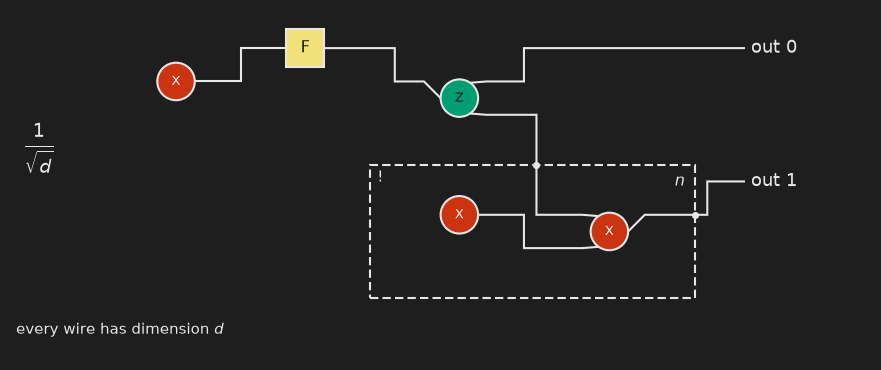
\includegraphics[width=0.75\textwidth]{figures/pictorial-ghzcircuit-dark.png}
\caption{The same drawing as PNG with the dark-theme defaults (ink \texttt{\#e6e6e6} on
\texttt{\#1e1e1e}), opaque, at density 1.5, as a terminal without color reports shows it.}
\label{fig:pictorial-dark}
\end{figure}

\subsection{W state}\label{sec:pictorial-ex-w}

The three-qubit W state~\cite{dur2000three} is a W node fed by an X spider with phase
$\tfrac12$ turn (the state $\ket{1}$):
\begin{lstlisting}[style=azx]
load
  p = X(0 -> 1, literal 2) phase{1: 1/2}
  w = W(1 -> 3, literal 2)
  p -> w
\end{lstlisting}

\begin{figure}[ht]
\centering
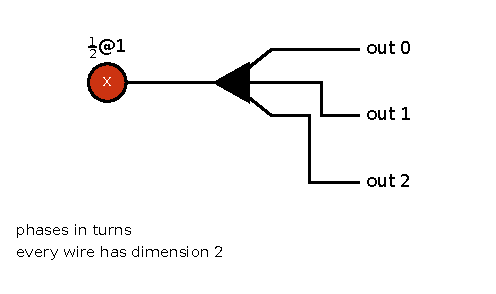
\includegraphics[width=0.42\textwidth]{figures/pictorial-wstate.pdf}\hfill
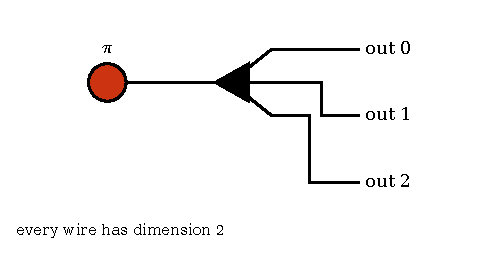
\includegraphics[width=0.42\textwidth]{figures/pictorial-wstate-pub.pdf}
\caption{The W state in normal mode (left, phase $\tfrac12$ in turns) and publication mode
(right, phase $\pi$).}
\label{fig:pictorial-wstate}
\end{figure}

The W node's three outputs spread over $\pm0.8h_b$ on its flat side; the outer two reach their
lanes by slanted segments.
\begin{lstlisting}[style=pgrid]
                ┎────out 0
                ┃
    Ⓧ1/2@1────◀W┠────out 1
                ┃
                ┖────out 2
phases in turns
every wire has dimension 2
\end{lstlisting}
\begin{lstlisting}[style=pgrid]
                   ]----out 0
                   ]
    (X 1/2@1)----<W]----out 1
                   ]
                   ]----out 2
phases in turns
every wire has dimension 2
\end{lstlisting}

\subsection{Generator gallery}\label{sec:pictorial-ex-gens}

A chain through an X spider with the phase family $-k/d$, a triangle, an inverse triangle, a
Fourier box, a weighted Z spider, and a discard shows most glyphs:
\begin{lstlisting}[style=azx]
load
  X(0 -> 1) phase{k: -k/d} -> T(d) -> Ti(d) -> F -> z = Z(1 -> 1) weight{1: a}
  z -> G(d)
\end{lstlisting}

\begin{figure}[ht]
\centering
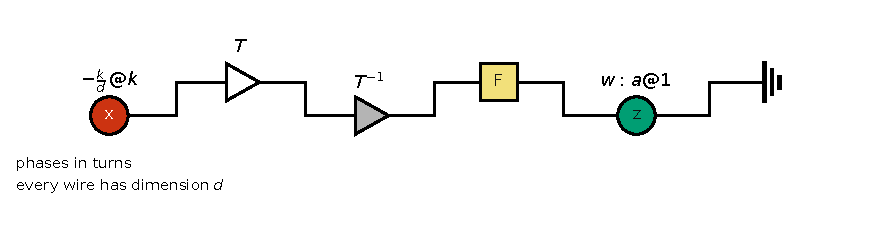
\includegraphics[width=0.85\textwidth]{figures/pictorial-gens.pdf}\\[2mm]
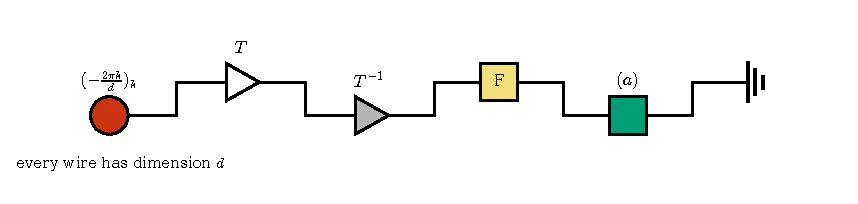
\includegraphics[width=0.85\textwidth]{figures/pictorial-gens-pub.pdf}
\caption{Generator gallery in normal mode (top) and publication mode (bottom). In publication
mode the weighted Z spider becomes a Z box with the coefficient vector $(a)$.}
\label{fig:pictorial-gens}
\end{figure}

\begin{lstlisting}[style=pgrid]
    Ⓧ-k/d @k────▷T────▶T⁻¹────[F]────Ⓩw: a@1────⏚
phases in turns
every wire has dimension d
\end{lstlisting}
\begin{lstlisting}[style=pgrid]
    (X -k/d @k)----|>T----|>T^-1----[F]----(Z w: a@1)----_|_
phases in turns
every wire has dimension d
\end{lstlisting}

\subsection{Splitter and binder}\label{sec:pictorial-ex-split}

A dimension splitter followed by a dimension binder carries three distinct wire dimensions, so
every wire is labeled in the margin of its first channel and no dimension note appears:
\begin{lstlisting}[style=azx]
load
  s = S(literal 2, literal 3)
  b = B(literal 2, literal 3)
  wire s.out0 -- b.in0
  wire s.out1 -- b.in1
\end{lstlisting}

\begin{figure}[ht]
\centering
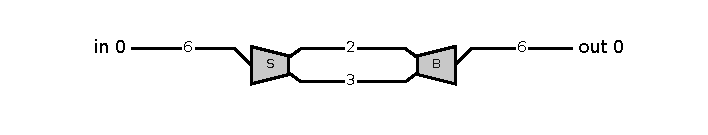
\includegraphics[width=0.7\textwidth]{figures/pictorial-split.pdf}
\caption{A splitter and a binder with labeled wire dimensions.}
\label{fig:pictorial-split}
\end{figure}

\begin{lstlisting}[style=pgrid]
    in 0──6───⊳S┎──2───┒⊲B──6───out 0
                ┃      ┃
                ┖──3───┚
\end{lstlisting}
\begin{lstlisting}[style=pgrid]
    in 0--6--->S]--2---[<B--6---out 0
                ]      ]
                ]--3---[
\end{lstlisting}
